\documentclass[12pt, a4paper, hidelinks]{article}

\usepackage{graphicx}
\usepackage{hyperref}
\usepackage{xcolor}
\usepackage[english]{babel}
\usepackage[nottoc]{tocbibind}
\usepackage[utf8]{inputenc}
\usepackage[T1]{fontenc}
\usepackage[style=verbose,backend=biber,style=authoryear, citestyle=authoryear ]{biblatex}
\addbibresource{ref.bib} % The filename of the bibliography
\usepackage[left=2.5cm,right=2.5cm,top=2.5cm,bottom=2.5cm]{geometry}
\usepackage{acronym}
\usepackage{fancyhdr}
\pagestyle{fancy}
\usepackage{lipsum}
\usepackage{array, tabularx, booktabs} % For better tables
\usepackage{booktabs}
\usepackage{multirow}
\usepackage{longtable}
%\usepackage{listings} % Code environments
%\usepackage{lstautogobble}  % Fix relative indenting
%\usepackage{color}          % Code coloring
%\usepackage{zi4}            % Nice font
\usepackage{minted}
\usemintedstyle{tango}
\setminted{linenos, autogobble, bgcolor=gray!5}
\usepackage{cleveref}
\usepackage{titlesec}
\setlength{\marginparwidth}{2cm}
\usepackage{todonotes}
\usepackage[autostyle=true]{csquotes}

\iffalse

\definecolor{codegreen}{rgb}{0,0.6,0}
\definecolor{codegray}{rgb}{0.5,0.5,0.5}
\definecolor{backcolour}{gray}{0.95}
\definecolor{codeorange}{rgb}{0.8,0.5,0.2}

\lstdefinestyle{mystyle}{
    backgroundcolor=\color{backcolour},  
    commentstyle=\color{codegray},
    keywordstyle=\color{codeorange},
    numberstyle=\tiny\color{codegray},
    stringstyle=\color{codegreen},
    basicstyle=\ttfamily\footnotesize,
    breakatwhitespace=false,         
    breaklines=true,                 
    captionpos=b,                    
    keepspaces=true,                 
    numbers=left,                    
    numbersep=5pt,                  
    showspaces=false,                
    showstringspaces=false,
    showtabs=false,                  
    tabsize=2
}

%\lstset{style=mystyle}

\definecolor{bluekeywords}{rgb}{0.13, 0.13, 1}
\definecolor{greencomments}{rgb}{0, 0.5, 0}
\definecolor{redstrings}{rgb}{0.9, 0, 0}
\definecolor{graynumbers}{rgb}{0.5, 0.5, 0.5}

\usepackage{listings}
\lstset{
    autogobble,
    columns=fullflexible,
    showspaces=false,
    showtabs=false,
    breaklines=true,
    showstringspaces=false,
    breakatwhitespace=true,
    escapeinside={(*@}{@*)},
    commentstyle=\color{greencomments},
    keywordstyle=\color{bluekeywords},
    stringstyle=\color{redstrings},
    numberstyle=\color{graynumbers},
    basicstyle=\ttfamily\footnotesize,
    frame=l,
    framesep=12pt,
    xleftmargin=12pt,
    tabsize=4,
    captionpos=b
}

\fi

\titleformat{\section}[hang]{\huge\bfseries}{\thesection\hspace{20pt}}{0pt}{\huge\bfseries}
\graphicspath{{Figures/}{./}{Assets/}}

% --- document configuration ---

\newcommand{\thesistitle}{Profiling tree species classification with synthetic data and deep learning}  
\newcommand{\supervisor}{Dorothea Sommer} 
\newcommand{\authorname}{Hauke Kirchner}
%\newcommand{\university}{Georg-August-Universität Göttingen}
%\newcommand{\department}{Institute of Computer Science}
\newcommand{\thesistype}{Seminar Report}
%\newcommand{\matrikelnumber}{[Put your matrikel number here]}
\newcommand{\keywords}{} % Set keywords that describe your report

\hypersetup{pdftitle=\thesistitle} % Set the PDF's title to your title
\hypersetup{pdfauthor=\authorname} % Set the PDF's author to your name
\hypersetup{pdfkeywords=\keywords} % Set the PDF's keywords to your keywords

\begin{document}

\fancyhead{}
\fancyhead[R]{\footnotesize \thesistitle}
\fancyfoot{}
\fancyfoot[R]{\thepage}
\fancyfoot[L]{Section \thesection}
\fancyfoot[C]{\authorname}
\renewcommand{\headrulewidth}{0.4pt}
\renewcommand{\footrulewidth}{0.4pt}

\pagestyle{plain}


    

% --- title page ---

\begin{titlepage}
\begin{minipage}[t]{0.6\textwidth}
\begin{flushleft}

\includegraphics[width=6.5cm]{logo-goettingen.pdf}
\end{flushleft}
\end{minipage}
\begin{minipage}[t]{0.4\textwidth}
\begin{center}
\qquad
\includegraphics[width=2.5cm]{hps-logo.pdf}
\end{center}
\end{minipage}

\begin{center}

\vspace*{.06\textheight}
\LARGE \thesistype\\[0.5cm]

\rule{.9\linewidth}{.6pt} \\[0.4cm] % Horizontal line
{\huge \bfseries \thesistitle}\vspace{0.4cm}
\rule{.9\linewidth}{.6pt} \\[1.5cm] % Horizontal line
 
\Large\authorname\\
\hfill\\
%\large MatrNr: \matrikelnumber\\ \vfill
Supervisor: \supervisor 
\vfill
%\university\\
%\department
\vfill
{\large \today}\\[4cm] % Date
 
\vfill
\end{center}
\end{titlepage}
    

% --- abstract ---

%\thispagestyle{empty}
\newpage
\pagenumbering{roman}
\setcounter{page}{1}

\section*{Abstract}


\medskip
\iffalse
General structure of an abstract, write 1 to 2 sentences per section
\begin{enumerate}
\item  A general statement introducing the broad research area of the particular topic being investigated.
\item  An explanation of the specific problem (difficulty, obstacle, challenge) to be solved.
\item  A review of existing or standard solutions to this problem and their limitations.
\item  An outline of the proposed new solution.
\item  A summary of how the solution was evaluated and what the outcomes of the evaluation were.
\end{enumerate}

You may find the following resources useful:
\begin{itemize}
    \item \url{https://www.grammarly.com/blog/write-an-abstract/}
    \item \url{https://www.editage.com/insights/manuscript-structure-how-to-convey-your-most-important-ideas-through-your-paper}
    \item More useful links: \url{https://hps.vi4io.org/teaching/ressources/start}
\end{itemize}
\fi

%\thispagestyle{empty}
% --- table of contents ---
% Comment out the lists you are not using
\newpage


\clearpage
\phantomsection\pdfbookmark{\contentsname}{toc}
\tableofcontents

\newpage
\clearpage\phantomsection
\listoftables
%\newpage
%\clearpage
\phantomsection
\listoffigures
%\newpage
%\clearpage
\phantomsection
\listoflistings \addcontentsline{toc}{section}{List of Listings}

% if you have abbreviations
\newpage

\section*{List of Abbreviations} \addcontentsline{toc}{section}{List of Abbreviations}
\begin{acronym}[Bash] % Add acronyms such that they are shown in full only on first occurrence
    \acro{HPC}{High-Performance Computing}
    \acro{FLOPS}{floating point operations per second}
    \acro{MACs}{multiply-accumulate operations}
    \acro{GPU}{Graphics processing unit}
    \acro{CPU}{Central processing unit}
\end{acronym}

\thispagestyle{plain}
\newpage

% --- content ---

\pagenumbering{arabic}
\setcounter{page}{1}
\pagestyle{fancy}


\section{Introduction}

\iffalse
Why is it important to benchmark the training process of neural networks?

1. Training speed
2. Energy efficiency -> GreenAI
\fi

Recent advances in deep learning made the technology more popular in several fields of research.
This lead to breakthroughs which helped to ...
Increasingly applications in forestry profit from deep learning applications and pubications in recent years have shown the great potential. Often traning data is a bottleneck for the application of neural networks. Especially in the field of environmental research collecting data requires substential effort. In Germany the largest effort to cellect data of German forests is the "Bundeswaldinventur". This involves the work of multiple teams over 

Especilly for lidar data of forests not to many pre-trained networks exist. Therfore, we test an approach where the pre-training is done based on synthetically generated lidar data representing individual trees.

Simultaniously, the emerging use of deep learning also leads to an increase in energy consumption. This phenomen studied by \cite{20220610_dodge_measuring-the-carbon-intensity-of-ai-in-cloud-instances}. 


\cite{white_2016_als-forest-inventory}
\cite{uba_2020_waldumbau}

\begin{itemize}
    \item Identify \textbf{profiling tools} that can help to \textbf{optimize an existing PyTorch workflow}.
    \item As this approach should help scientists, the \textbf{usibility is of high importance}. The simplest tool for doing the job is preferred.
    \item In contrast to training benchmark suites, such as MLPerf, I do not focus on benchmarking hardware but on optimizing an existing PyTorch workflow (viewpoint of a scientist)
\end{itemize}

\iffalse
The introduction is the most important part of such a report. Its general structure is similar to the Abstract but with about one paragraph per section as listed again below.
\begin{enumerate}
\item  A general statement introducing the broad research area of the particular topic being investigated.
\item  An explanation of the specific problem (difficulty, obstacle, challenge) to be solved.
\item  A review of existing or standard solutions to this problem and their limitations.
\item  An outline of the proposed new solution.
\item  A summary of how the solution was evaluated and what the outcomes of the evaluation were.
\end{enumerate}
Furthermore, the introduction should have a contributions section, that summarizes, possibly as a list, what the report and the work described in the report has contributed.
Finally, the introduction should end with an outline of the remaining report.

\ac{HPC} refers to the usage of powerful compute systems to solve non-trivial problems.

\subsection{Citation and figure example}
Hawthorn et al. \cite{20220610_dodge_measuring-the-carbon-intensity-of-ai-in-cloud-instances} talk about laser, which is similar to the work of his colleagues \cite{20220610_dodge_measuring-the-carbon-intensity-of-ai-in-cloud-instances, 20220610_dodge_measuring-the-carbon-intensity-of-ai-in-cloud-instances}.
\begin{figure}[th]
\centering

\includegraphics[width=0.7\textwidth]{speed_FILL0_wght400_GRAD0_opsz48.png}
\caption[An Electron]{An electron (artist's impression).}
\label{fig:Electron}
\end{figure}

\subsection{Table and listing example}
\Cref{tab:treatments} shows an example for a table in \LaTeX.
\begin{table}[th]
\label{tab:treatments}
\centering
\begin{tabularx}{0.45\textwidth}{l||r|r}
Groups & Treatment X & Treatment Y \\
\hline \hline
1 & 0.20 & 0.80\\
2 & 0.17 & 0.70\\
3 & 0.24 & 0.75\\
4 & 0.68 & 0.30\\
\end{tabularx}
\caption{The effects of treatments X and Y on the four groups studied.}
\end{table}

[If you show results in tables, always ensure all of them are aligned to the right and have the same precision.]

\Cref{lst:hello} shows an example of a listing, a good way to display code in \LaTeX.

\begin{listing}
\begin{minted}{Go}
package main
import "fmt"
func main() {
    fmt.Println("Hello, world!")
}
\end{minted}
\caption{"Hello, world!" in Go}
\label{lst:hello}
\end{listing}
\fi

\iffalse
\begin{lstlisting}[language=Go, caption={"Hello, world!" in Go}, label=lst:hello]
package main
import "fmt"
func main() {
    fmt.Println("Hello, world!")
}
\end{lstlisting}
\fi

\section{Methods}
\label{sec:methods}

\subsection{Tree species classification based on synthetic lidar data}
\label{sec:workflow}

The use case for testing profiling options available for PyTorch is lidar-based tree species classification. 
Recently, several applications of deep learning approaches for analyzing lidar data were proposed (~\cite{2017_qi_pointnet, 2021_krisanski_fsct}).
As the computation cost for 3D convolutions is high, analyzing a workflow for lidar data processing is an ideal real world example explore the capabilities of profilers for PyTorch.

In the project ForestCare~\footnote{https://hps.vi4io.org/research/projects/forestcare/start, accessed on: 13.03.2023} a pre-training workflow based on synthetic lidar data was developed, to overcome the lack of available pre-trainined neural networks for tree species classification.
A detailed description of this workflow can be found in~\Cref{fig:lidar-workflow}.
The code for pre-training the poinet model can be found in the accompanying github repository~\footnote{\url{https://github.com/haukekirchner/scap/}, accessed on: 22.02.2023}.


\begin{figure}[H]
\centering
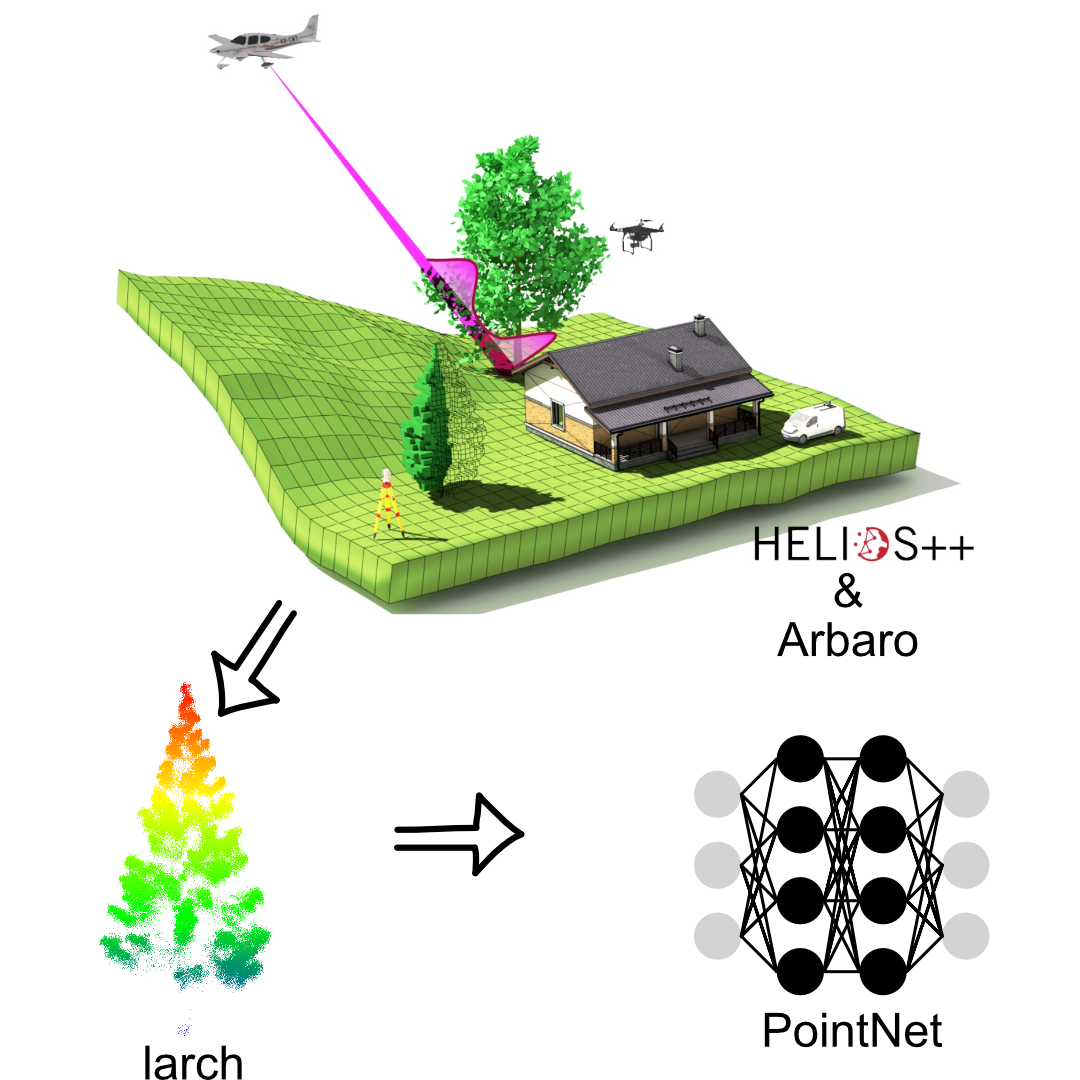
\includegraphics[width=0.5\textwidth]{assets/workflow_synthetic_data}
\caption[Workflow for generating synthetic lidar data ]{The workflow for generating synthtic lidar data starts with the generation of tree models. This is done with the software Arbaro\footnote{\url{https://github.com/wdiestel/arbaro}, accessed on: 22.02.2023}~(\cite{weber_1995_arbaro}). Based on these models Helios++~(\cite{9906068}) is used to simulate lidar data which is similar to data capture with the Zenmuse L1 sensor from dji~\footnote{\url{https://www.dji.com/de/zenmuse-l1}, accessed on: 22.02.2023}. Following this generated data is used to pre-train a PointNet model proposed by ~\textcite{2017_qi_pointnet}. The figure is adapted from \textcite{9906068}.}
\label{fig:lidar-workflow}
\end{figure}

\subsection{Fundamentals of software profiling}
\label{sec:profiling}

% general introduction
Software profiling is "a form of dynamic program analysis (as opposed to static code analysis), is the investigation of a program's behavior using information gathered as the program executes"~(\cite{wiki:profiling}).
Metrices that are commonly of interest to identify performance bottlenecks are the number and the elapsed time per function call, as well as the memory consumption.

% definition of metrics
Metrics traditionally used for software profiling are execution time and \acf{FLOPS}~(\Cref{tab:metrics}).
Execution time is a simple measure, which reports on the total time a function call takes.
\ac{FLOPS} refers to the number of floating point operations that can be executed per second and can be used to evalute the models efficiency.

With the advent of \ac{GPU}'s throughput and \acf{MACs} gained importance~(\cite{verma_2019_metrics-ml-benchmarking}).
Throughput is of high importance as deep learning models need to analyze massive amounts of data to finde generalizable patterns and can report on the models speed.
As "most of modern hardware architectures uses FMA [fused multiply-add] instructions for operations with tensors.  FMA computes $a*x+b$ as one operation. Roughly $GMACs = 0.5 * GFLOPs$"\footnote{\url{https://github.com/sovrasov/flops-counter.pytorch/issues/16\#issuecomment-518585837} , accessed on: 22.11.2022}.


Additionally, the PyTorch Profiler tracks the memory consumption. As deep learning applications depend on massive amounts of data, the effective usage of \ac{GPU}'s internal memory is critical to the overall performance.

Further important profiling measure in deep learing, which are not considered in this report, are Time to Accuracy (TTA) and Average Time to Multiple Thresholds (ATTMT)~(\cite{verma_2019_metrics-ml-benchmarking}).

% Please add the following required packages to your document preamble:
% \usepackage{booktabs}
% \usepackage{multirow}
\begin{table}[H]
\centering
\begin{tabular}{@{}ll@{}}
\toprule
metric                                                                                 & purpose                        \\ \midrule
Execution time                                                                         & \multirow{2}{*}{traditionally} \\
FLOPS                                                                                  &                                \\ \midrule
Throughput: $\frac{images}{sec}$                                                       & \multirow{2}{*}{with the advent of GPUs} \\
MACs                                                                                   &                                \\ \bottomrule
\end{tabular}
\caption[Overview of performance metrics]{Overview of performance metrics which were used for profiling.}
\label{tab:metrics}
\end{table}



\subsection{Overview of profiling tools}
\label{sec:tools-overview}

Many different profiling tools that could be used to gain insights into the PyTorch workflow presented in~\Cref{sec:workflow} exist (a small collection can be found in~\Cref{tab:tools}).
General profiling tools such as Intel's Vtune~\footnote{\url{https://www.intel.com/content/www/us/en/developer/tools/oneapi/vtune-profiler.html}, accessed on: 22.11.2022} or the open-source software LIKWID\footnote{\url{https://github.com/RRZE-HPC/likwid}, accessed on: 22.11.2022} can be used to collect useful metrices of any software.

However, for PyTorch tools were developed specifically to the needs one need to profile PyTorch workflows.
One popular tool is the in-build PyTorch profiler, which can be used in combination with tensorboard~\footnote{\url{https://www.tensorflow.org/tensorboard/}, accessed on: 16.03.2023}. This graphical visualization can both be used for beginners and experts to optimize their workflows, as it provides performance recommendations, as well as detailed metrics such as the call stack or the trace view.
Another tool that was specifically designed for PyTorch is Deepspeed~\footnote{\url{https://www.deepspeed.ai/tutorials/flops-profiler/}, accessed on: 16.03.2023}. Here specifically the FlopsProfiler was used, as the Pytorch Profiler lacks the option to analyze FLOPS.


General profiling tools could not provide automatic recommendations and as useful visualisations to highlight critical aspects, as they do not have the insights into PyTorch. Consequently more expert knowledge is required to make good use of tools like LIKWID or Vtune.
As one of the reasearch goals of this project was the identification of eas-to-use tools this report focuses on the PyTorch Profiler and the Deepspeed's FlopsProfiler.


pytorch tutorial \footnote{\url{https://pytorch.org/tutorials/intermediate/tensorboard_profiler_tutorial.html}, accessed on: 22.11.2022}

% Please add the following required packages to your document preamble:
% \usepackage{booktabs}
% \usepackage{multirow}
\begin{table}[H]
\centering
\begin{tabular}{@{}lll@{}}
\toprule
tool                              & metrics                                                                                & scope                    \\ \midrule
\href{https://pytorch.org/tutorials/intermediate/tensorboard_profiler_tutorial.html}{PyTorch Profiler With TensorBoard} & \begin{tabular}[c]{@{}l@{}}performance metrics\\ (e.g. time, memory)\end{tabular}      & \multirow{2}{*}{PyTorch} \\
\href{https://www.deepspeed.ai/tutorials/flops-profiler/}{Deepspeed/FlopsProfiler}                      & FLOPS                                                                                  &                          \\ \midrule
\href{https://www.intel.com/content/www/us/en/developer/tools/oneapi/vtune-profiler.html}{Vtune}                             & \multirow{2}{*}{\begin{tabular}[c]{@{}l@{}}general\\ performance metrics\end{tabular}} & Intel-only               \\
\href{https://github.com/RRZE-HPC/likwid}{likwid}                            &                                                                                        & general                  \\ \bottomrule
\end{tabular}
\caption[Overview of profiling tools]{Ovierview of tools used for profiling.}
\label{tab:tools}
\end{table}


\subsection{Tensorboard}
\label{sec:Tensorboard}

\begin{listing}[H]
\inputminted[xleftmargin=1em,linenos,fontsize=\small, highlightlines={1,3,9-12,14-16}]{python}{./assets/tensorboard.py}
\caption[Code example for Tensorboard]{Highlighted parts of the code are required to use Tensorboard for profiling the training process of the neural network.}
\label{lst:tensorboard}
\end{listing}

\subsection{PyTorch - Profiler}
\label{sec:m-pytorch-profiler}

\begin{listing}[H]
\inputminted[breaklines, xleftmargin=1em,linenos,fontsize=\small, highlightlines={4-10,14,15}]{python}{./assets/profiler-torch.py}
\caption[Code example for PyTorch - Profiler]{Highlighted parts of the code are required to use the PyTorch Profiler for profiling the training process of the neural network.}
\label{lst:profiler-torch}
\end{listing}

\subsection{Deepspeed - FLOPSProfiler}
\label{sec:m-FLOPSprofiler}


\begin{listing}[H]
\inputminted[xleftmargin=1em,linenos,fontsize=\small, highlightlines={1,3,4,8,9,11-18}]{python}{./assets/deepspeed.py}
\caption[Code example for Deepspeed - FLOPSProfiler]{Highlighted parts of the code are required to use Deepspeed - FLOPSProfiler for profiling the training process of the neural network.}
\label{lst:deepspeed}
\end{listing}

\subsection{Experiments}
\label{sec:m-experiments}

\begin{figure}[H]
\centering
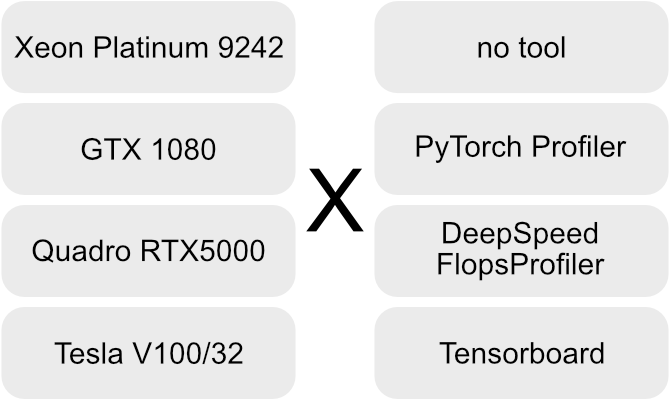
\includegraphics[width=0.5\textwidth]{./assets/experiments.png}
\caption[Overview of the runs]{In total 16 different runs where planned by testing all possible combinations of tools with available \ac{GPU}s and one \ac{CPU}. Four more runs where performed by adding some experiments according the data loader process and different batch sizes (\Cref{tab:experiments-all}).}
\label{fig:experiments}
\end{figure}

\begin{table}[H]
\label{tab:experiments-all}
\begin{tabular}{@{}llllll@{}}
\toprule
run & node         & tool           & job\_id  & is\_valid & experiment     \\ \midrule
1   & scc\_cpu     & no-tool        & 14629421 & TRUE      &                \\
2   & scc\_cpu     & tensorboard    & 14629426 & TRUE      &                \\
3   & scc\_cpu     & profiler-torch & 14650740 & TRUE      &                \\
4   & scc\_cpu     & deepspeed      & 14617521 & FALSE     &                \\
5   & scc\_gtx1080 & no-tool        & 14619617 & TRUE      &                \\
6   & scc\_gtx1080 & tensorboard    & 14615343 & TRUE      &                \\
7   & scc\_gtx1080 & profiler-torch & 14650076 & TRUE      &                \\
8   & scc\_gtx1080 & deepspeed      & 14615344 & TRUE      &                \\
9   & scc\_rtx5000 & no-tool        & 14619618 & TRUE      &                \\
10  & scc\_rtx5000 & tensorboard    & 14617172 & TRUE      &                \\
11  & scc\_rtx5000 & profiler-torch & 14650079 & TRUE      &                \\
12  & scc\_rtx5000 & deepspeed      & 14617171 & TRUE      &                \\
13  & scc\_v100    & no-tool        & 14619619 & TRUE      &                \\
14  & scc\_v100    & tensorboard    & 14617203 & TRUE      &                \\
15  & scc\_v100    & profiler-torch & 14650080 & TRUE      &                \\
16  & scc\_v100    & deepspeed      & 14617202 & TRUE      &                \\
17  & scc\_gtx1080 & profiler-torch & 14650758 & TRUE      & batch-size-64  \\
18  & scc\_gtx1080 & profiler-torch & 14650750 & TRUE      & sample-points  \\
19  & scc\_cpu     & profiler-torch & 14657599 & TRUE      & sample-points  \\
20  & scc\_gtx1080 & profiler-torch & 14650759 & TRUE      & batch-size-128 \\ \bottomrule
\end{tabular}
\caption[Ovierview over all runs including experiments]{In total 20 different experiments where performed. The first 16 experiments are directly derived from the experiment design presented in \Cref{fig:experiments}. Experiments 18 and 19 where done as preliminary work, to optimize the data loading process before all experiments are performed (~\Cref{sec:r-data-loading}). Experiments 17 and 20 where done based on the PyTorch - Profiler's performance recommendations(~\Cref{sec:r-pytorch-profiler}).}
\end{table}

footnote \footnote{\url{https://www.gwdg.de/web/guest/hpc-on-campus/scc} (Accessed on: 22.02.2023)}

\section{Results}
\label{sec:results}

\subsection{Optimization of the data loading process}
\label{sec:r-data-loading}



\begin{figure}[H]
\centering
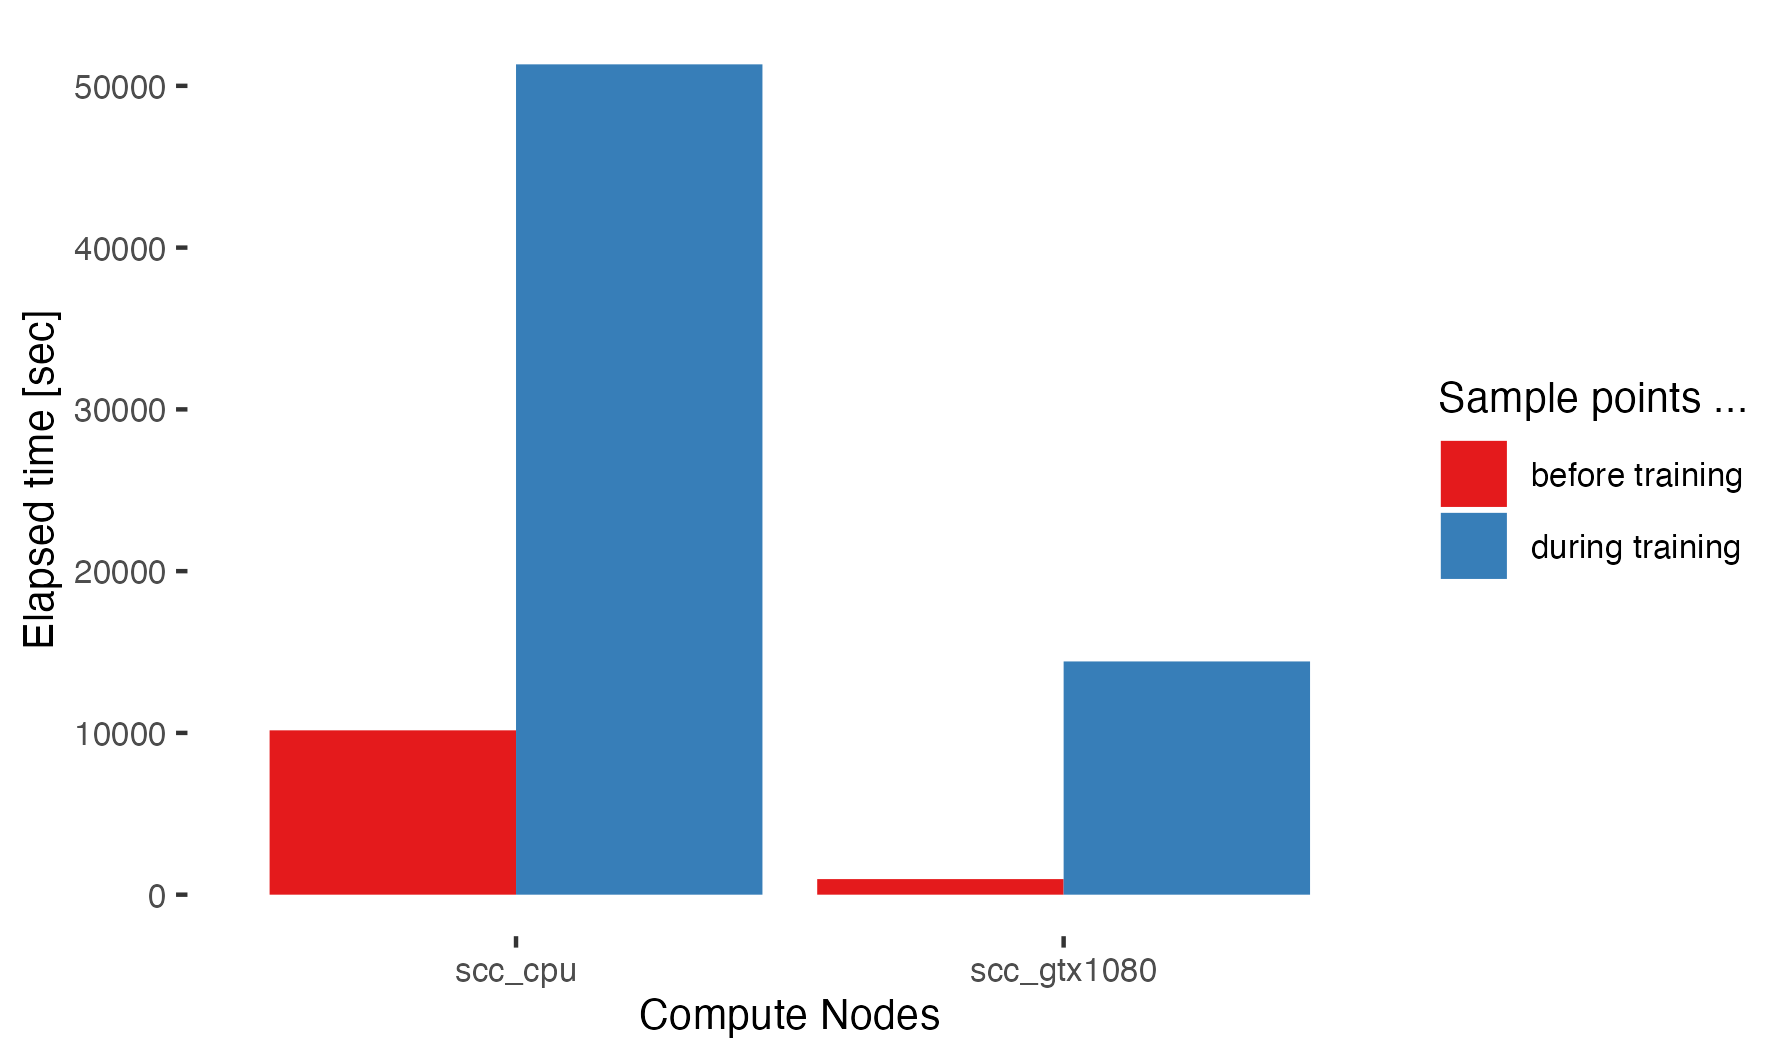
\includegraphics[width=0.5\textwidth]{./assets/sacct_barplot_by_nodes_sample-points-effect}
\caption[Data loading optimization]{By migrating the point sampling process from the data loader to a pre-processing step the elapsed time for the training runs was decreased significantly.}
\label{fig:sacct_barplot_by_nodes_sample-points-effect}
\end{figure}

\subsection{Runtime}
\label{sec:r-runtime}

\begin{figure}[H]
\centering
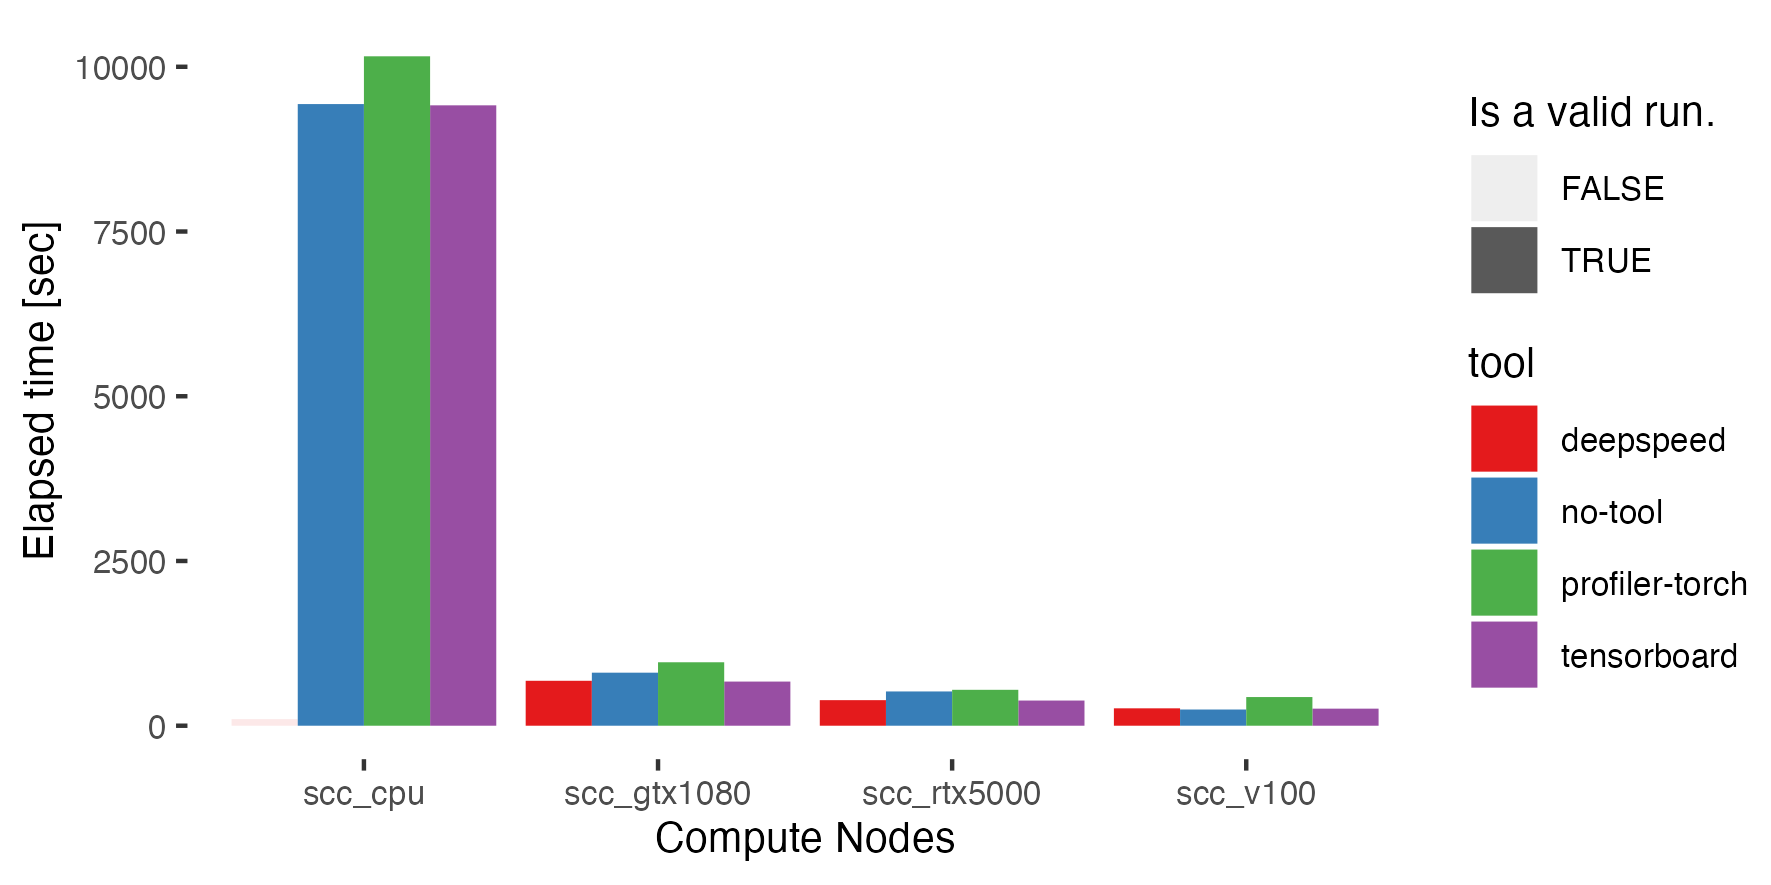
\includegraphics[width=1\textwidth]{./assets/sacct_barplot_by_nodes_no-experiment}
\caption[Runtime of the experiments]{The runtime of all runs testing the combintation of tools and \ac{GPU} and \ac{CPU} partitions (\Cref{fig:experiments}). }
\label{fig:sacct_barplot_by_nodes_no-experiment}
\end{figure}

\begin{figure}[H]
\centering
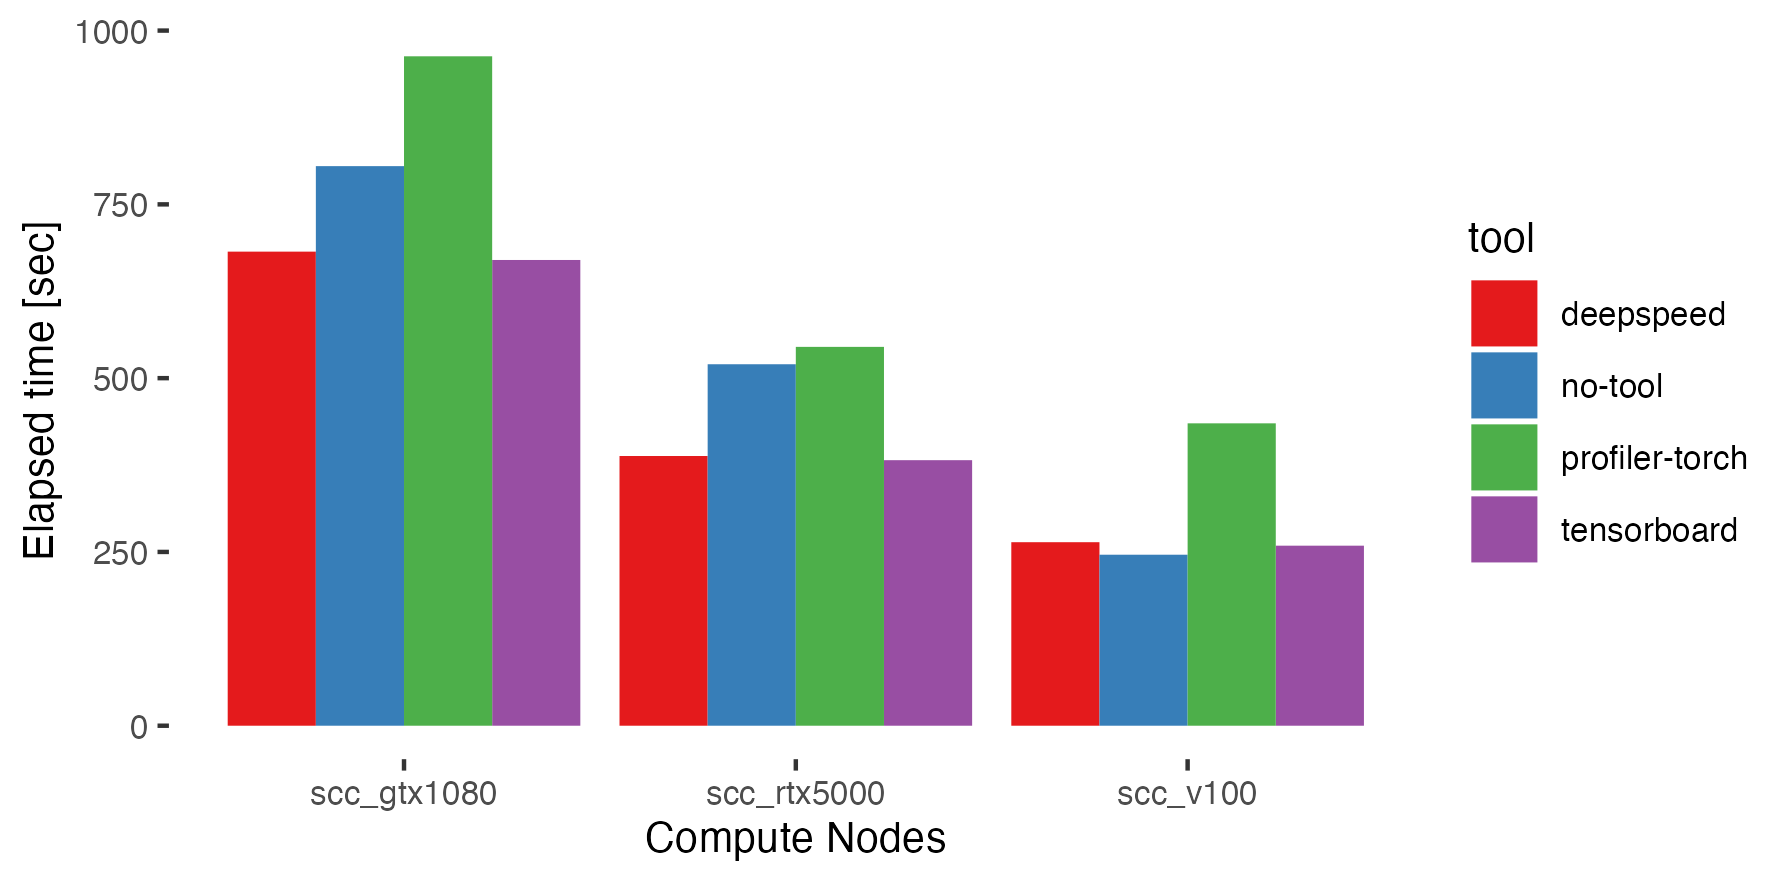
\includegraphics[width=1\textwidth]{./assets/sacct_barplot_by_nodes_no-experiment_gpu}
\caption[Runtime of the experiments (GPU-only)]{The runtime of all runs testing the combintation of tools and \ac{GPU} partitions - excluding \ac{CPU} partitions (\Cref{fig:experiments}).}
\label{fig:sacct_barplot_by_nodes_no-experiment_gpu}
\end{figure}

\subsection{PyTorch - Profiler}
\label{sec:r-pytorch-profiler}

\begin{figure}[H]
\centering
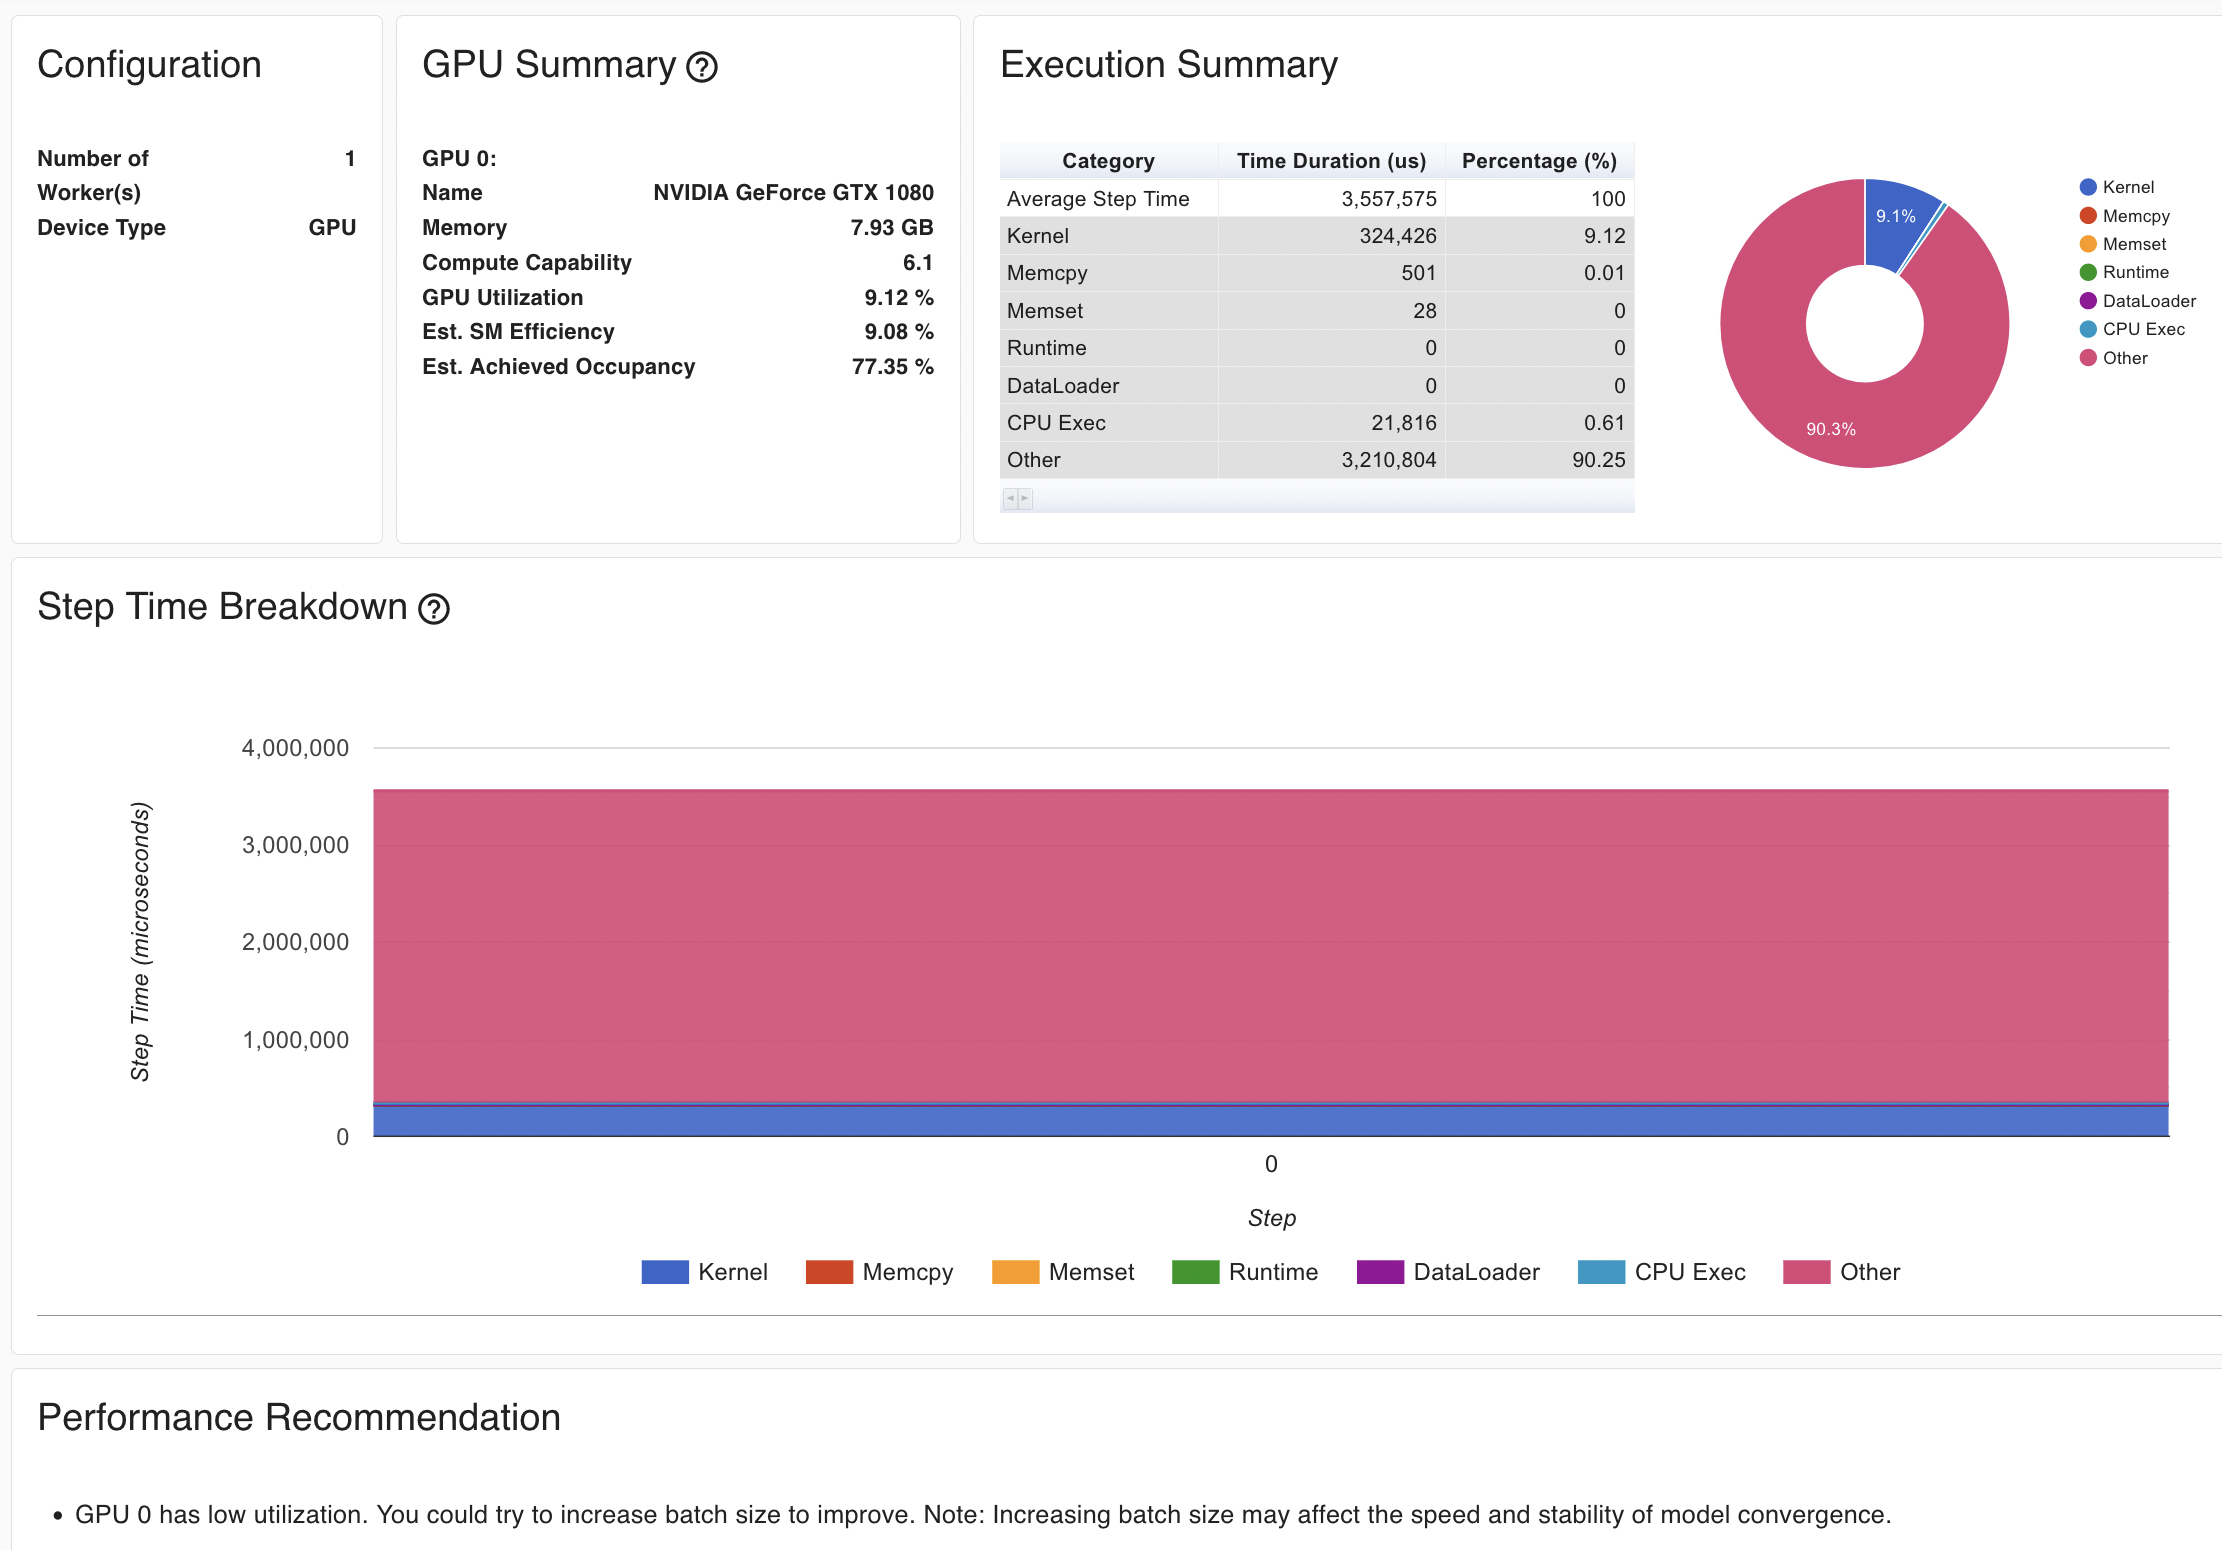
\includegraphics[width=1\textwidth]{./assets/scap_gtx1080_profiler-torch_14650076}
\caption[PyTorch - Profiler: Overview]{Visualizing the profiling results of the PyTorch - Profiler with Tensorboard provides an overview page. This page summarizes important metrics of the workflow, such as \ac{GPU} utilization. Details on the metrics can be found in the corresponding Github repository~\footnote{\url{https://github.com/pytorch/kineto/blob/main/tb_plugin/docs/gpu_utilization.md}, accessed on: 27.22023}. Further, it offers performance recommendations on how to adress potential bottlenecks. }
\label{fig:scap_gtx1080_profiler-torch_14650076}
\end{figure}

\begin{figure}[H]
\centering
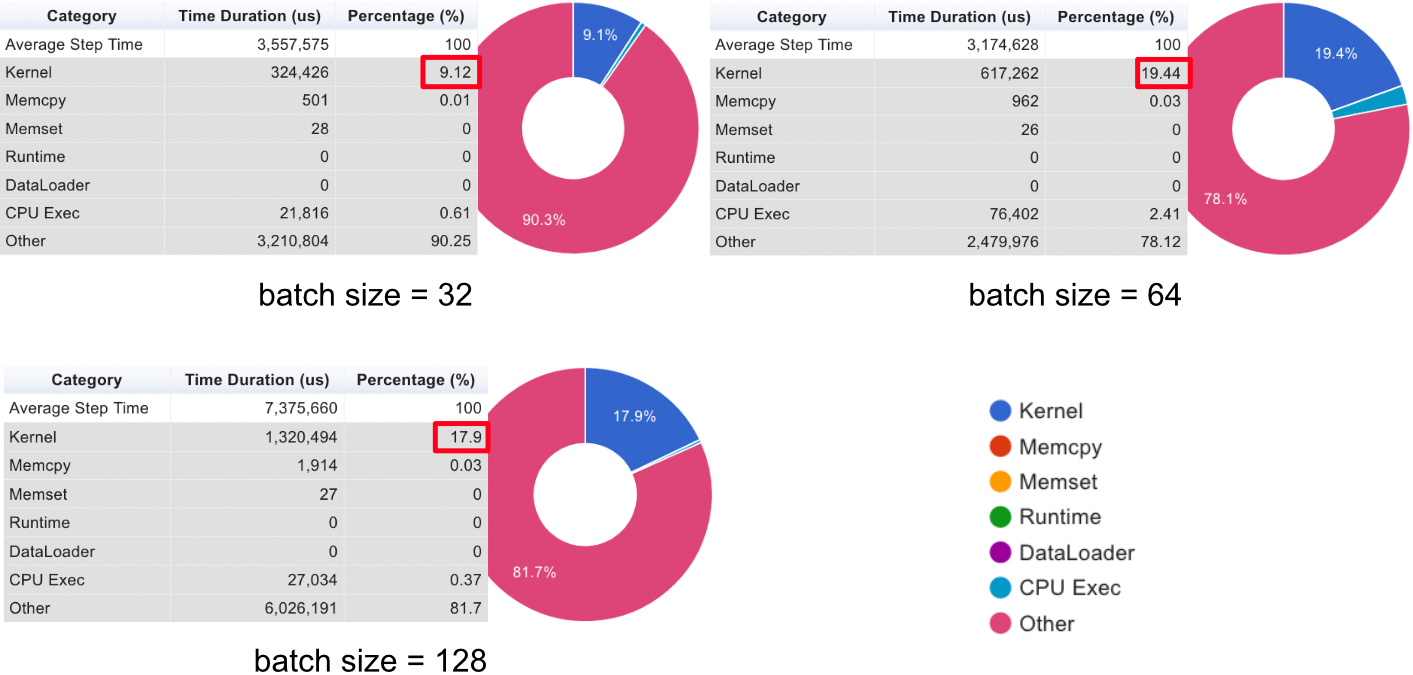
\includegraphics[width=1\textwidth]{./assets/scap_gtx1080_profiler-torch_comparison-batch-size}
\caption[PyTorch - Profiler: Performance Recommendation]{For the tested training workflow the performance recommendations of the PyTorch - Profiler suggest to increase the batch size. The effect of the batch size on the \ac{GPU} utilization can be seen for a batch size of 32 (run 7 in~\Cref{tab:experiments-all}), 64 (run 17 in~\Cref{tab:experiments-all}), 128 (run 20 in~\Cref{tab:experiments-all}).}
\label{fig:scap_gtx1080_profiler-torch_comparison-batch-size}
\end{figure}

\begin{figure}[H]
\centering
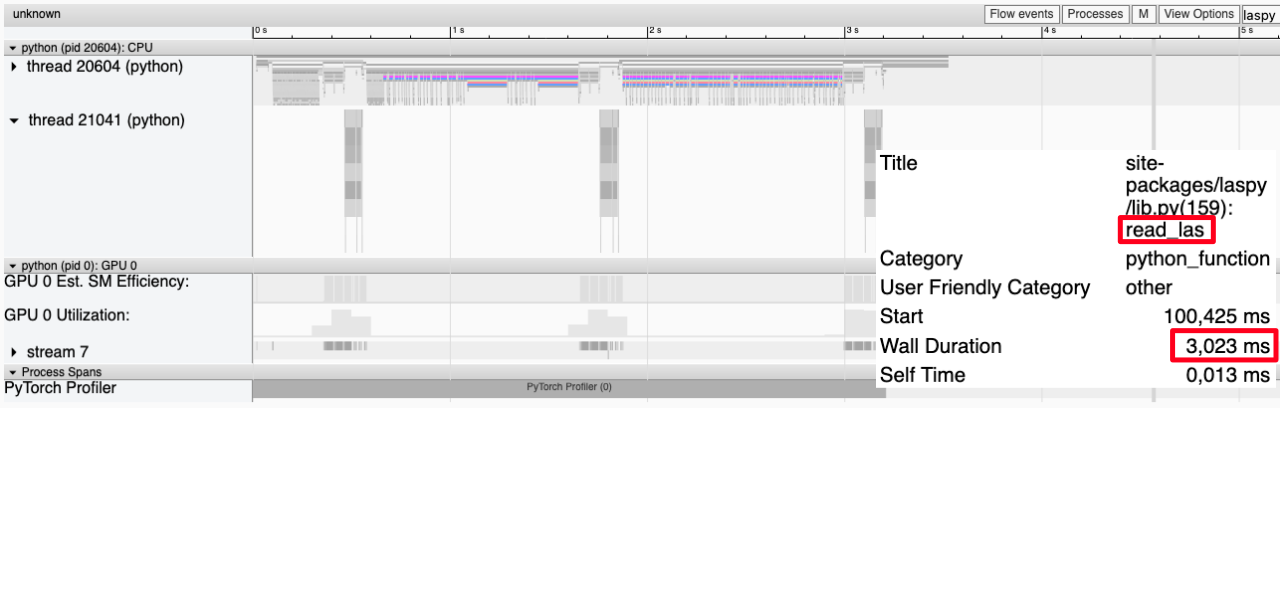
\includegraphics[width=1\textwidth]{./assets/scap_gtx1080_profiler-torch_batch-size-64_14650758_trace-view-laspy}
\caption*{Trace View: Laspy with presampled lidar data}
\label{fig:scap_gtx1080_profiler-torch_batch-size-64_14650758_trace-view-laspy}
\end{figure}

\begin{figure}[H]
\centering
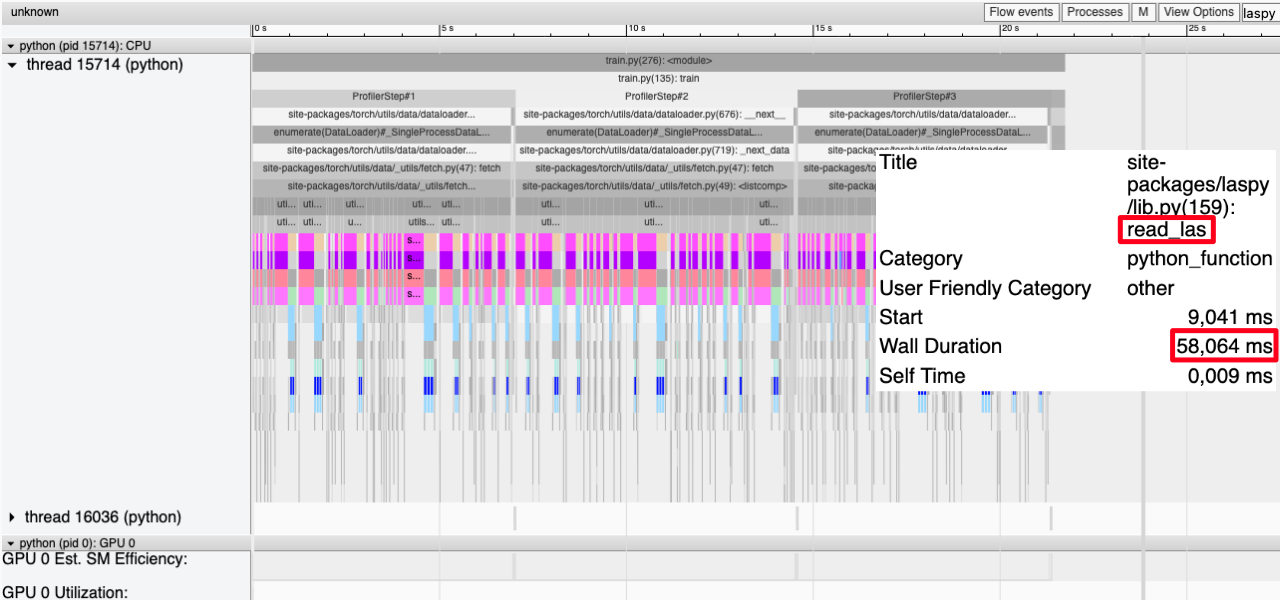
\includegraphics[width=1\textwidth]{./assets/scap_gtx1080_profiler-torch_sample-points_14650750_trace-view-laspy}
\caption*{Trace View: Laspy with raw lidar data}
\label{fig:scap_gtx1080_profiler-torch_sample-points_14650750_trace-view-laspy}
\end{figure}



\subsection{Deepspeed - FLOPSProfiler}
\label{sec:r-FLOPSprofiler}


\begin{listing}[H]
\inputminted[xleftmargin=1em,linenos,fontsize=\scriptsize, firstline=1,lastline=16]{python}{./assets/scap_gtx1080_deepspeed_14615344_4294967294_one-epoch.txt}
\caption{Summary}
\label{lst:scap_gtx1080_deepspeed_14615344_4294967294_one-epoch-summary}
\end{listing}

\begin{listing}[H]
\inputminted[xleftmargin=1em,linenos,fontsize=\scriptsize, firstline=18,lastline=31]{python}{./assets/scap_gtx1080_deepspeed_14615344_4294967294_one-epoch.txt}
\caption{Aggregated Profile per GPU}
\label{lst:scap_gtx1080_deepspeed_14615344_4294967294_one-epoch-aggregated}
\end{listing}

\begin{listing}[H]
\inputminted[xleftmargin=1em,linenos,fontsize=\tiny, firstline=33,lastline=48, breaklines]{python}{./assets/scap_gtx1080_deepspeed_14615344_4294967294_one-epoch.txt}
\caption{Detailed Profile per GPU}
\label{lst:scap_gtx1080_deepspeed_14615344_4294967294_one-epoch-detailed}
\end{listing}

\section{Discussion}
\label{sec:discussion}



\section{Conclusion}
\label{sec:conclusion}



% --- references ---

\newpage
\printbibliography[heading=bibintoc]

% --- your appendix ---
\appendix
\break

\pagenumbering{arabic}
\renewcommand*{\thepage}{A\arabic{page}}

\begin{figure}[H]
\centering
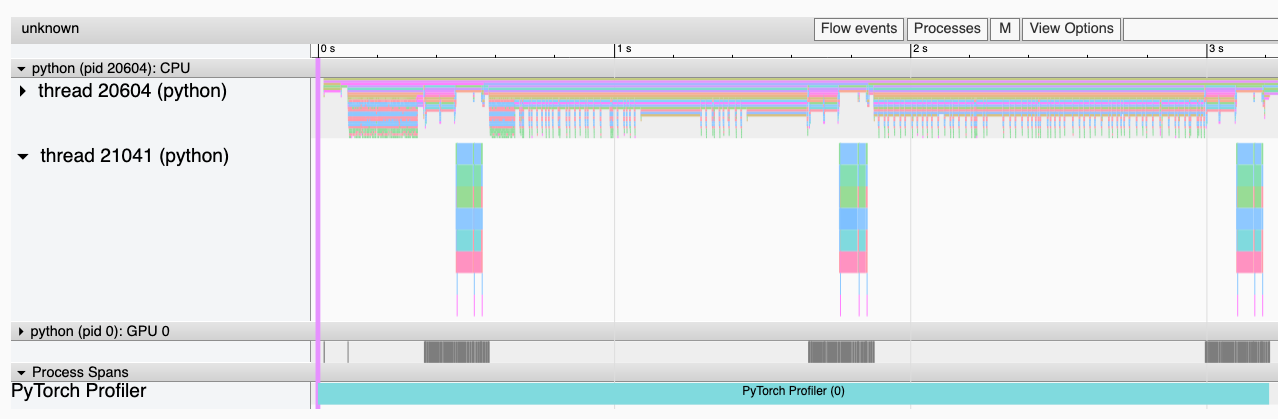
\includegraphics[width=1\textwidth]{./assets/scap_gtx1080_profiler-torch_batch-size-64_14650758_trace-view}
\caption*{Trace View}
\label{fig:scap_gtx1080_profiler-torch_batch-size-64_14650758_trace-view}
\end{figure}

\begin{figure}[H]
\centering
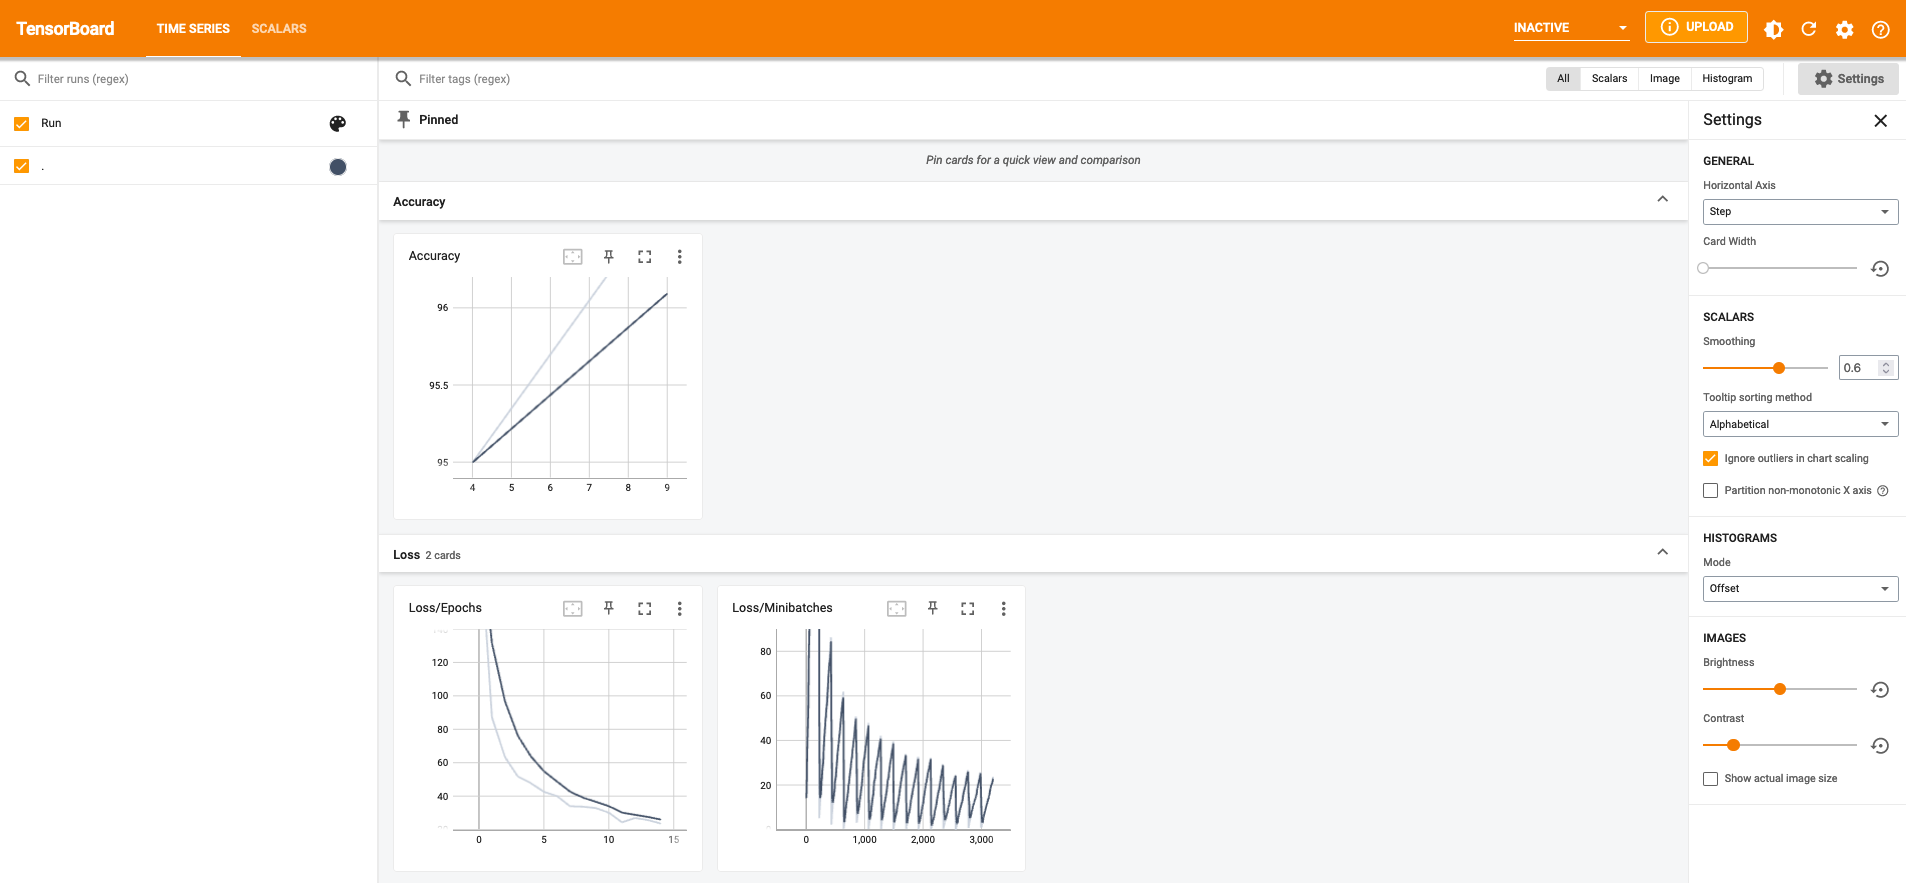
\includegraphics[width=1\textwidth]{./assets/scap_gtx1080_tensorboard_14615343}
\caption*{Tensorboard for run with GTX1080}
\label{fig:scap_gtx1080_tensorboard_14615343}
\end{figure}

\begin{figure}[H]
\centering
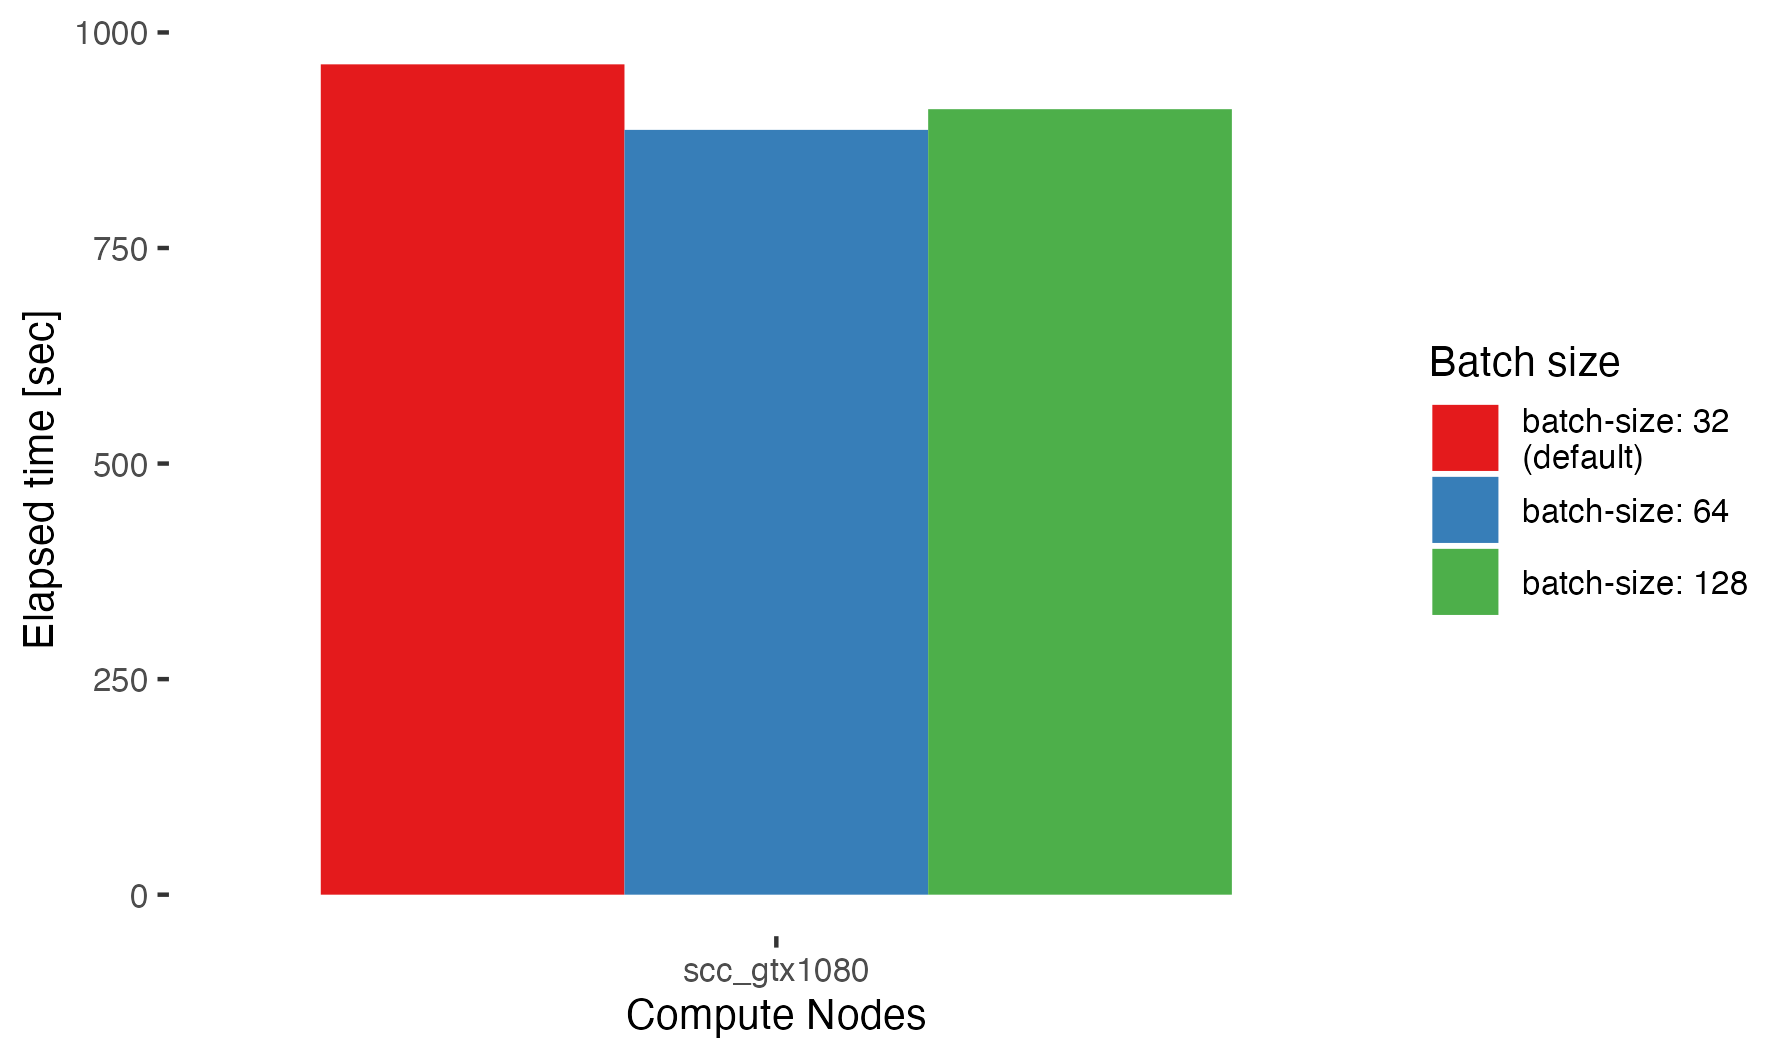
\includegraphics[width=0.85\textwidth]{./assets/sacct_barplot_by_nodes_batch-size-effect}
\caption*{result of increasing batch size on walltime}
\label{fig:sacct_barplot_by_nodes_batch-size-effect}
\end{figure}

\begin{figure}[H]
\centering
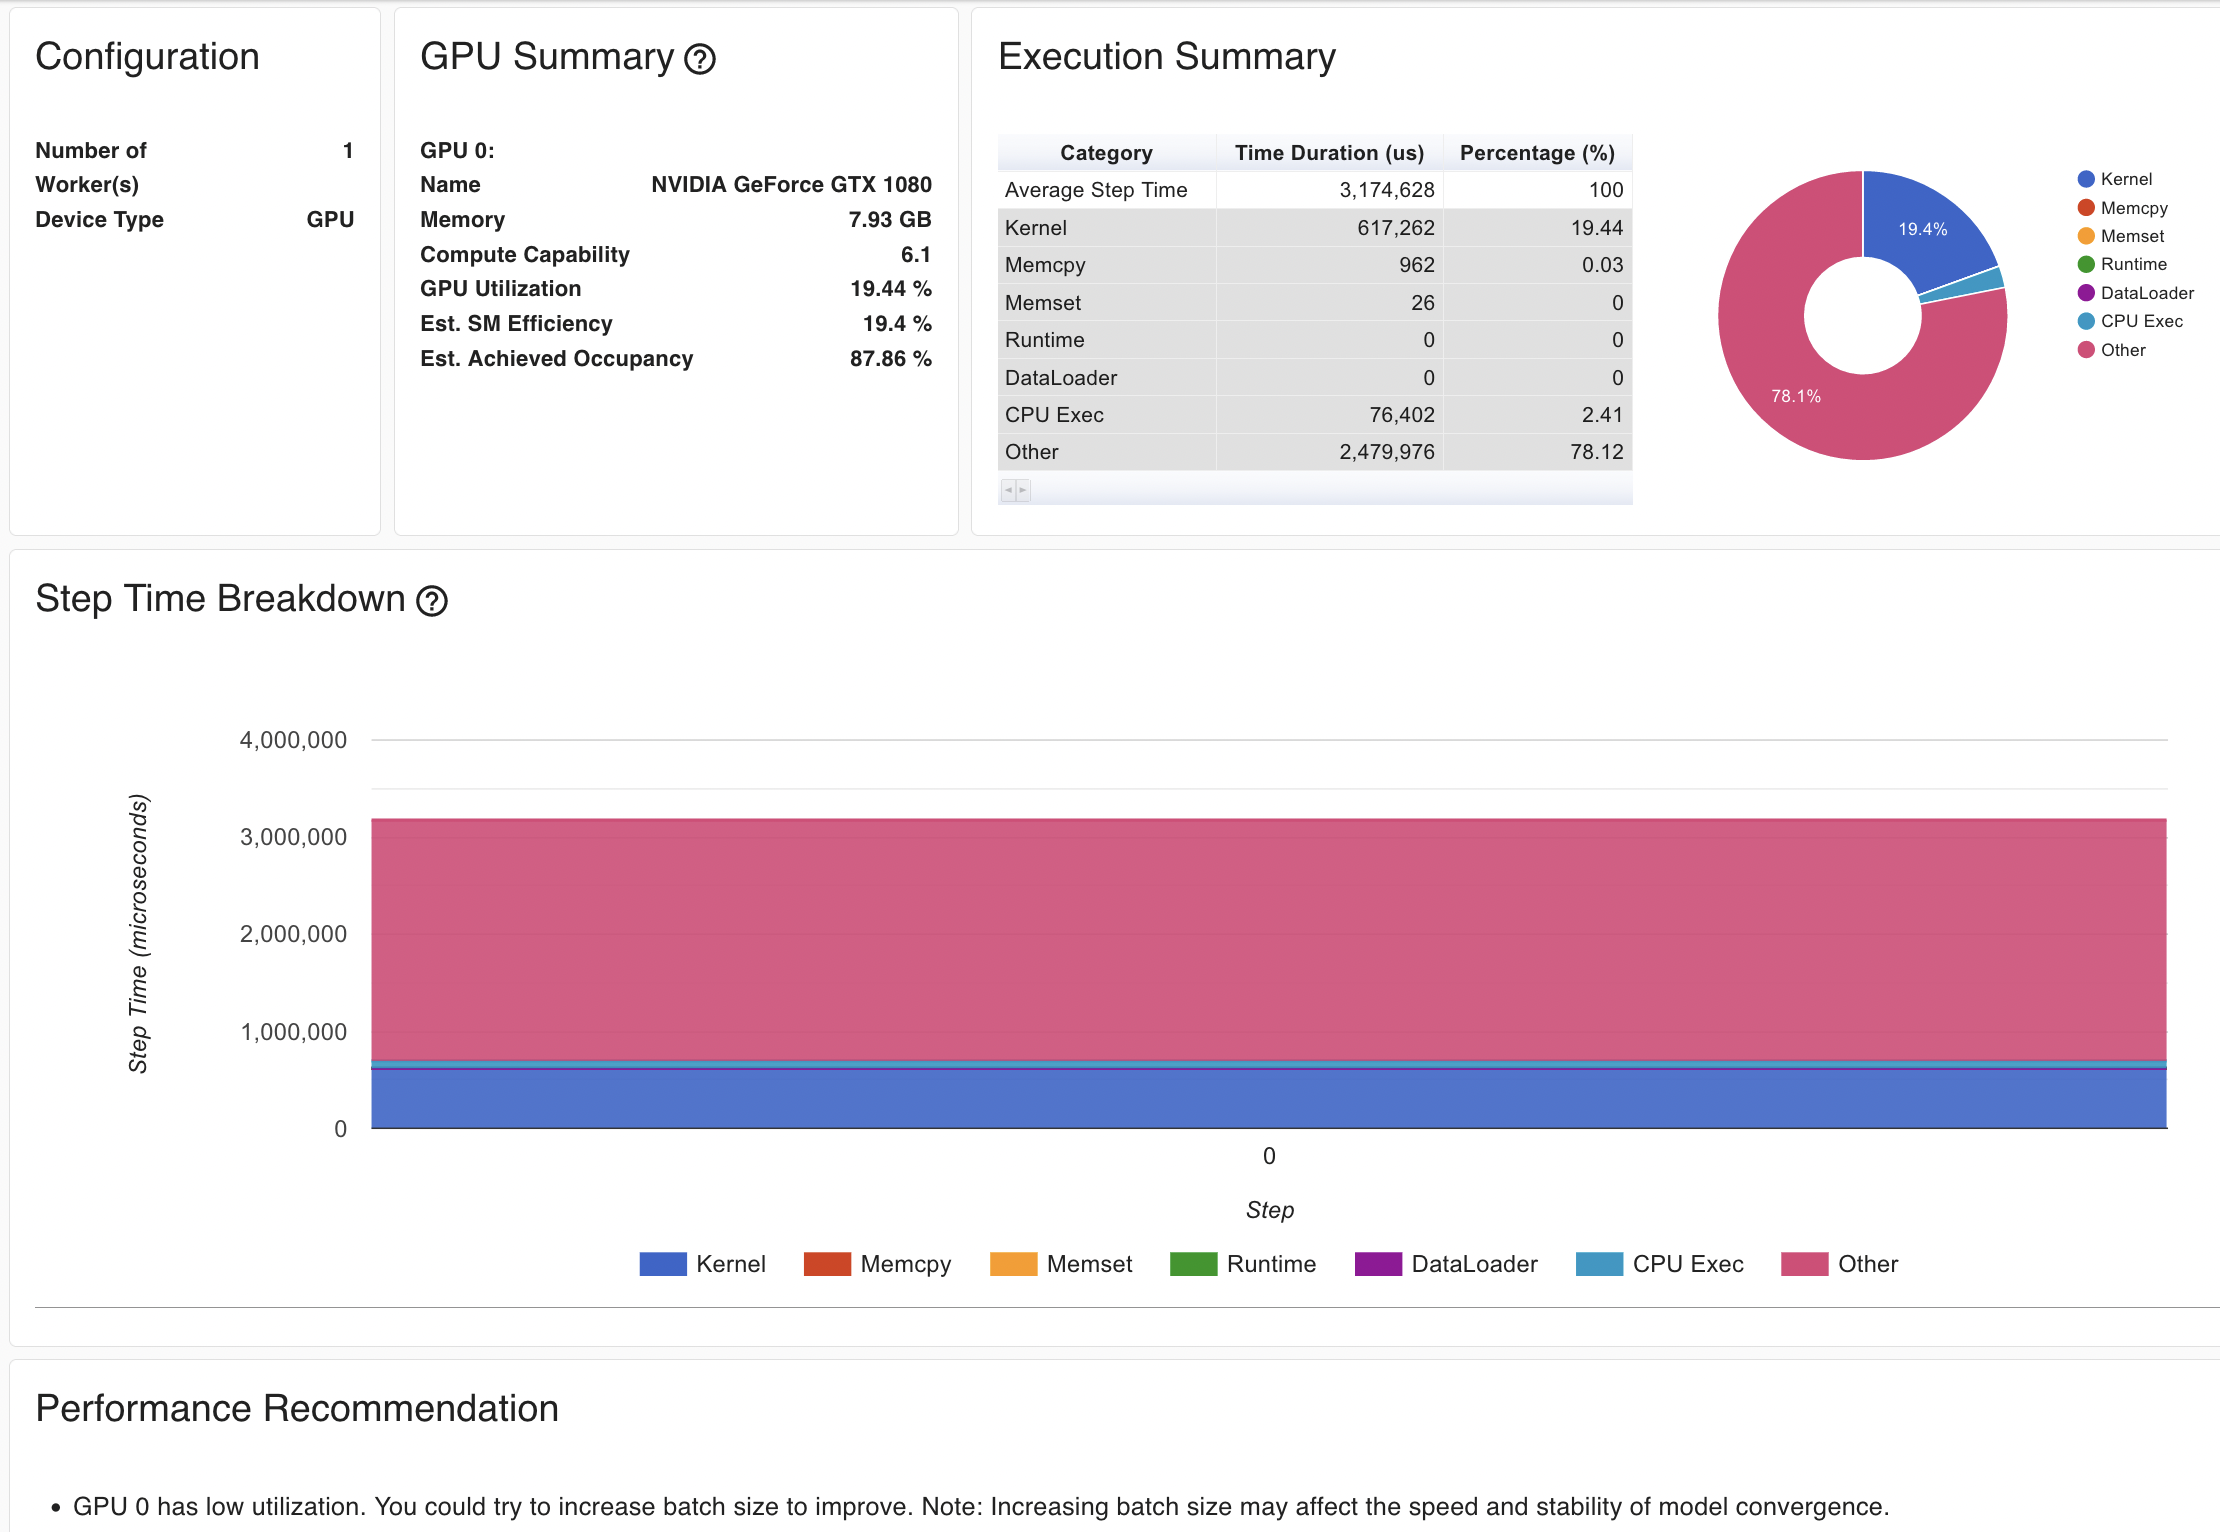
\includegraphics[width=0.7\textwidth]{./assets/scap_gtx1080_profiler-torch_batch-size-64_14650758}
\caption[test]{Overview: Increased batch size (64)}
\label{fig:scap_gtx1080_profiler-torch_batch-size-64_14650758}
\end{figure}

\begin{figure}[H]
\centering
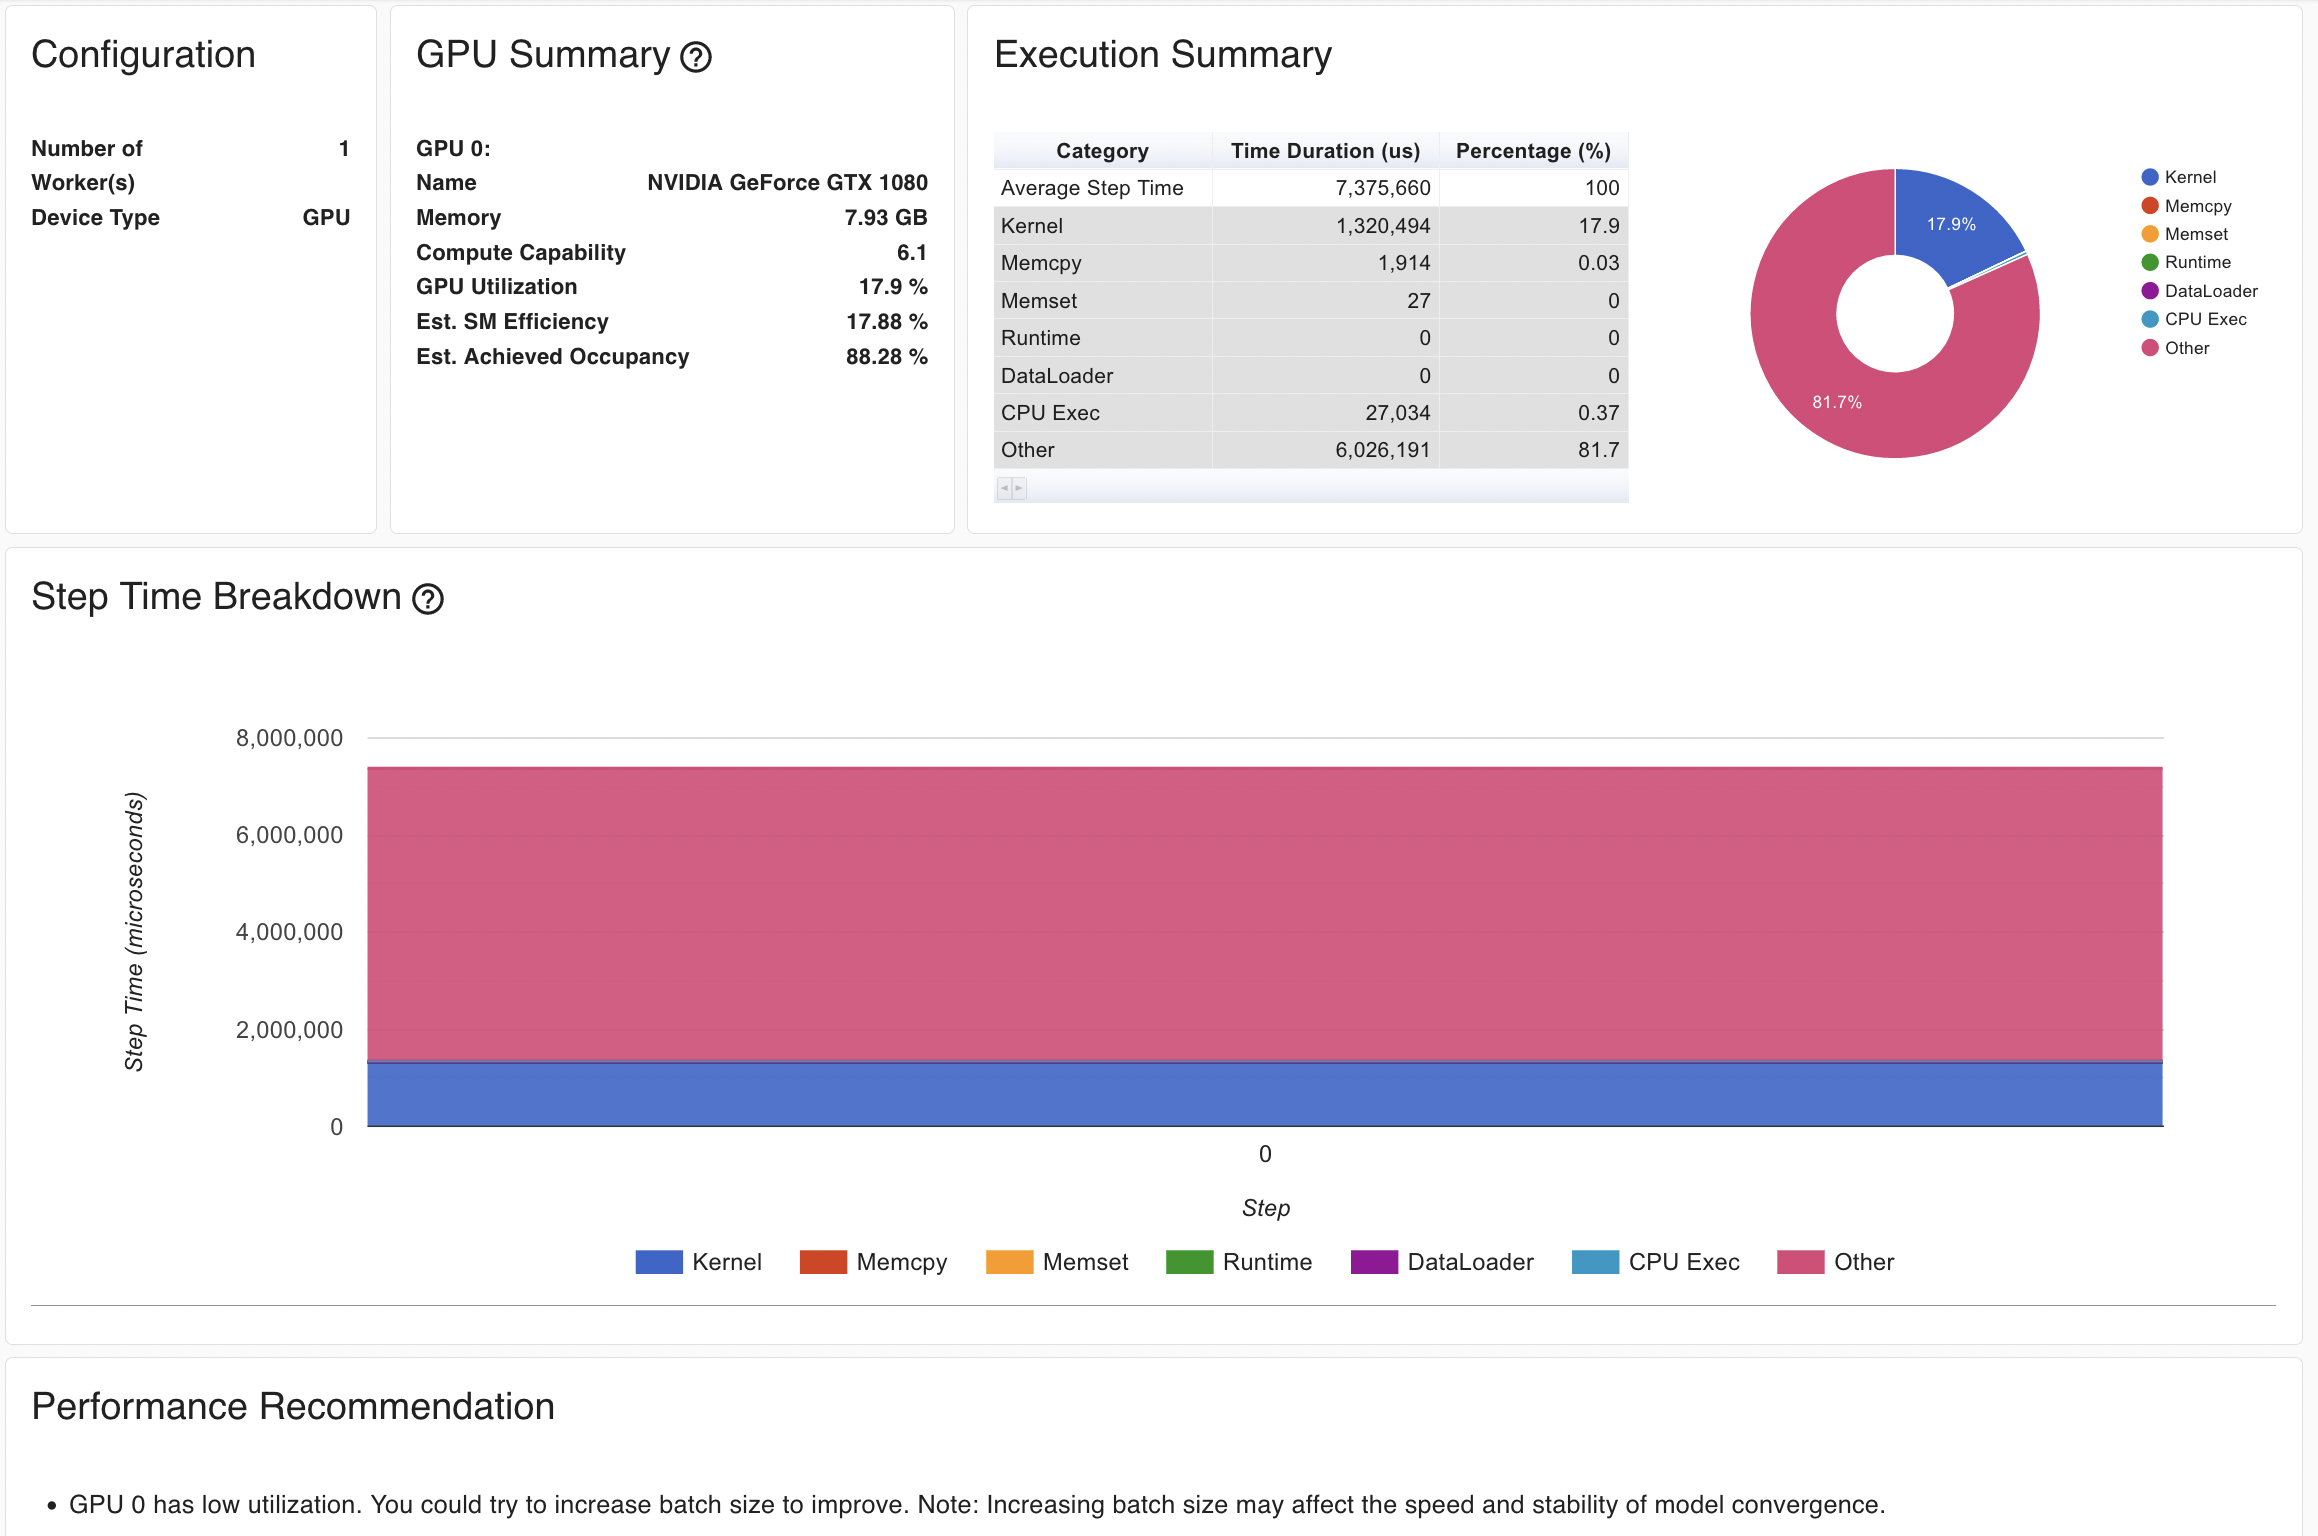
\includegraphics[width=0.7\textwidth]{./assets/scap_gtx1080_profiler-torch_batch-size-128_14650759}
\caption[]{Overview: Increased batch size (128)}
\label{fig:scap_gtx1080_profiler-torch_batch-size-128_14650759}
\end{figure}

\begin{figure}[H]
\centering
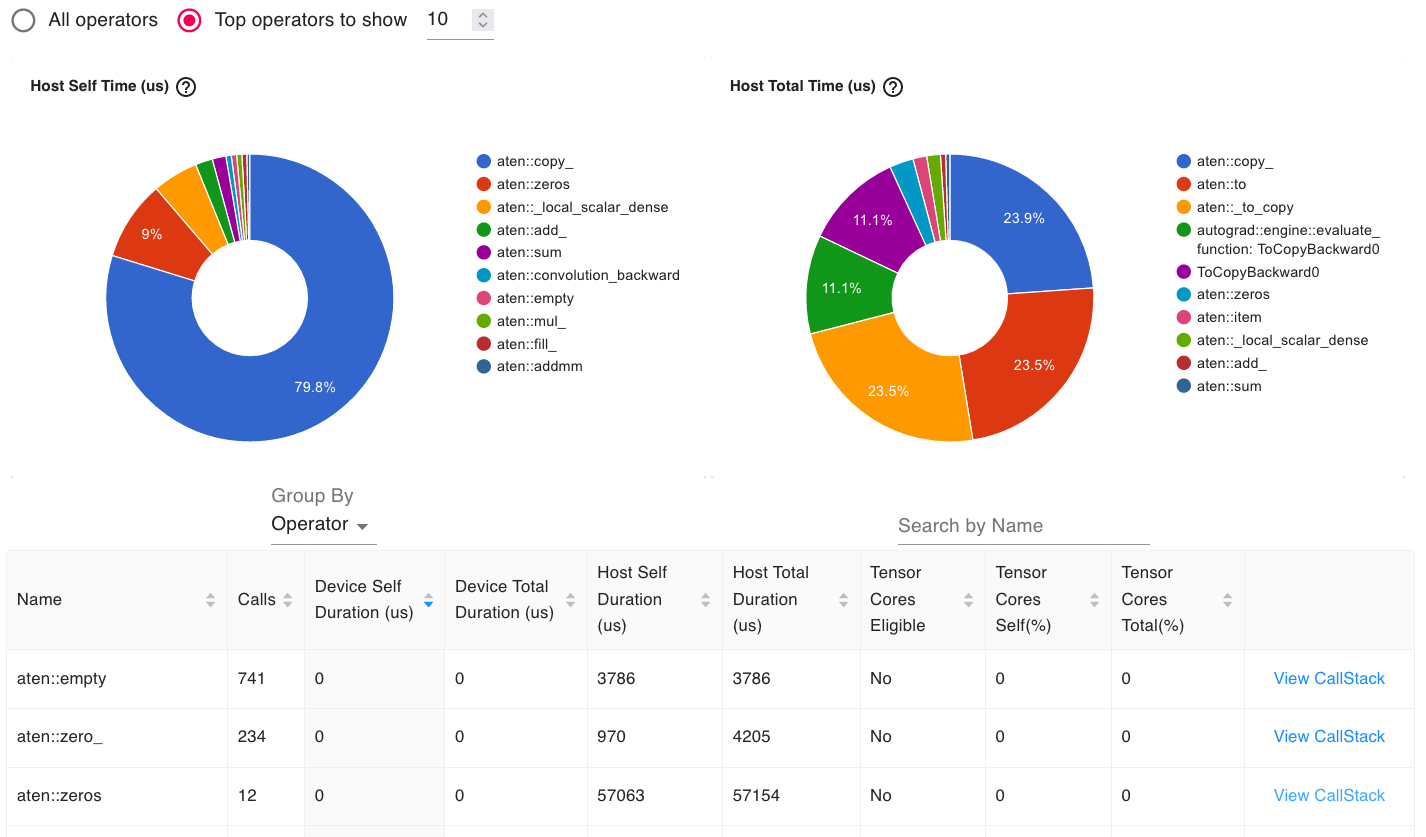
\includegraphics[width=0.9\textwidth]{./assets/scap_gtx1080_profiler-torch_batch-size-64_14650758_operator-view}
\caption[Operator View]{}
\label{fig:scap_gtx1080_profiler-torch_batch-size-64_14650758_operator-view}
\end{figure}

\begin{figure}[H]
\centering
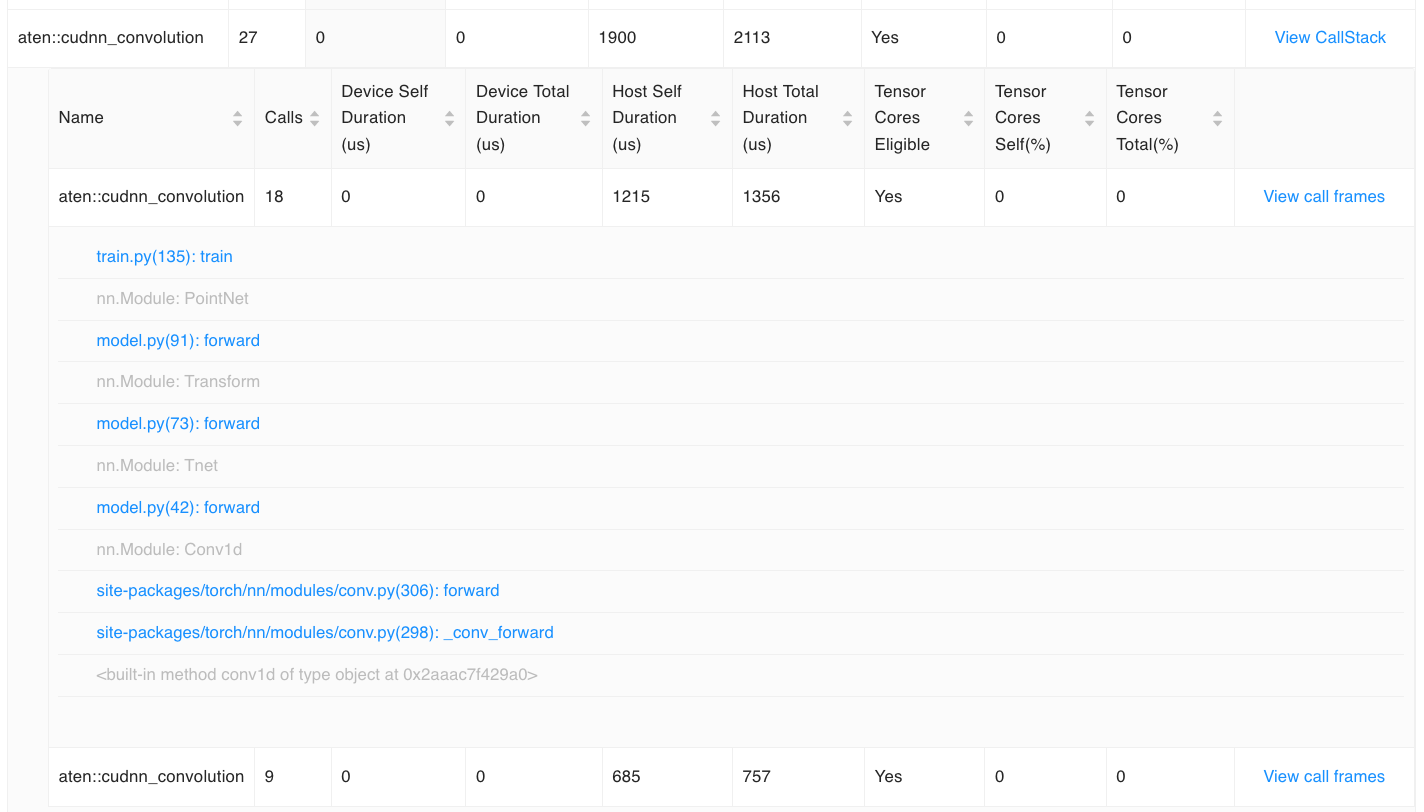
\includegraphics[width=0.9\textwidth]{./assets/scap_gtx1080_profiler-torch_batch-size-64_14650758_operator-view-details}
\caption[Operator View - Details]{}
\label{fig:scap_gtx1080_profiler-torch_batch-size-64_14650758_operator-view-details}
\end{figure}

\begin{figure}[H]
\centering
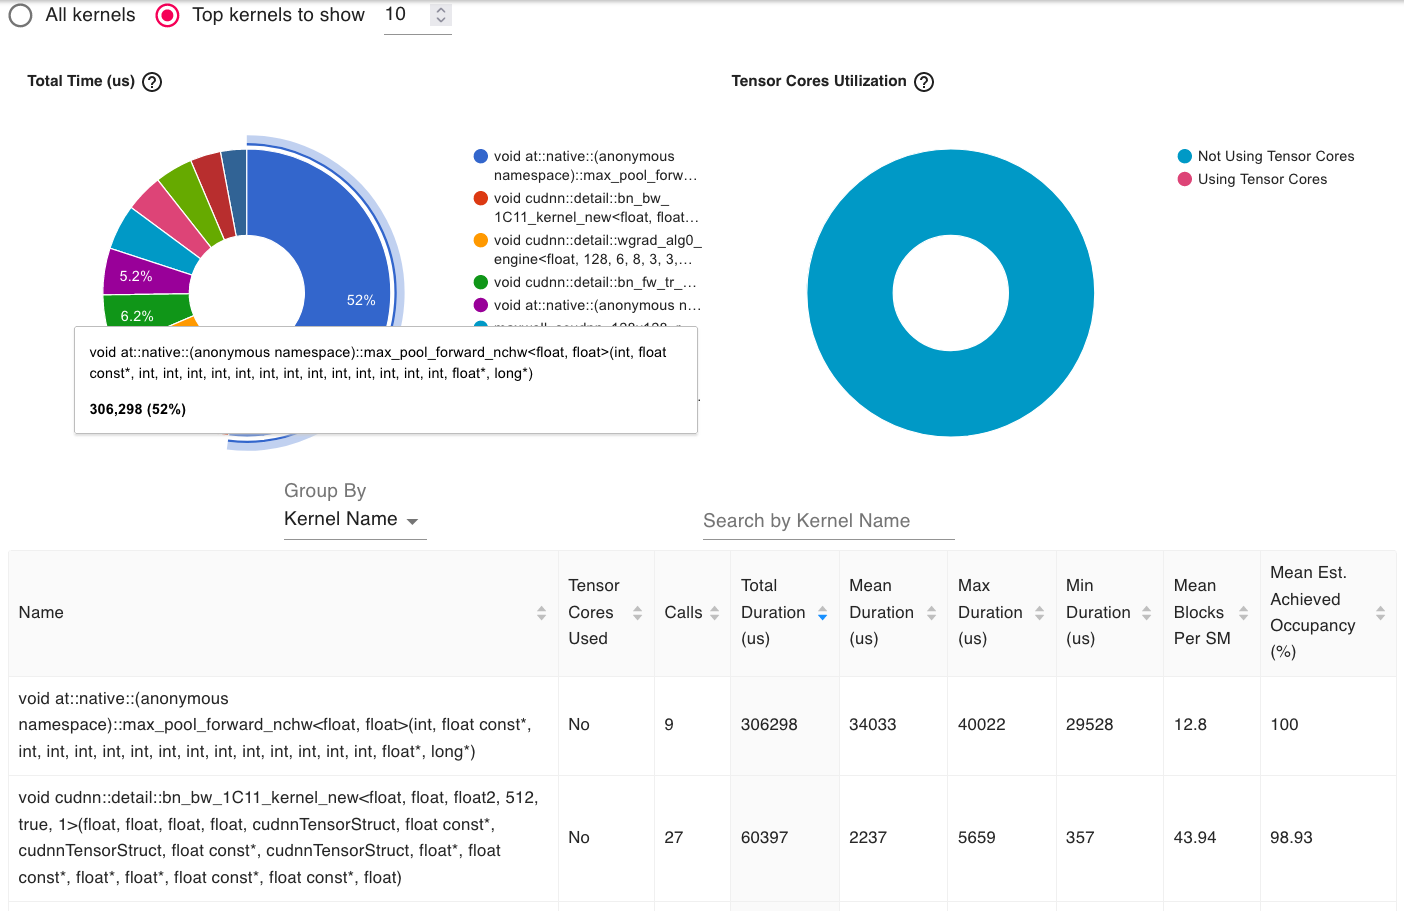
\includegraphics[width=0.9\textwidth]{./assets/scap_gtx1080_profiler-torch_batch-size-64_14650758_gpu-kernel-view}
\caption[GPU Kernel View]{}
\label{fig:scap_gtx1080_profiler-torch_batch-size-64_14650758_gpu-kernel-view}
\end{figure}

\begin{figure}[H]
\centering
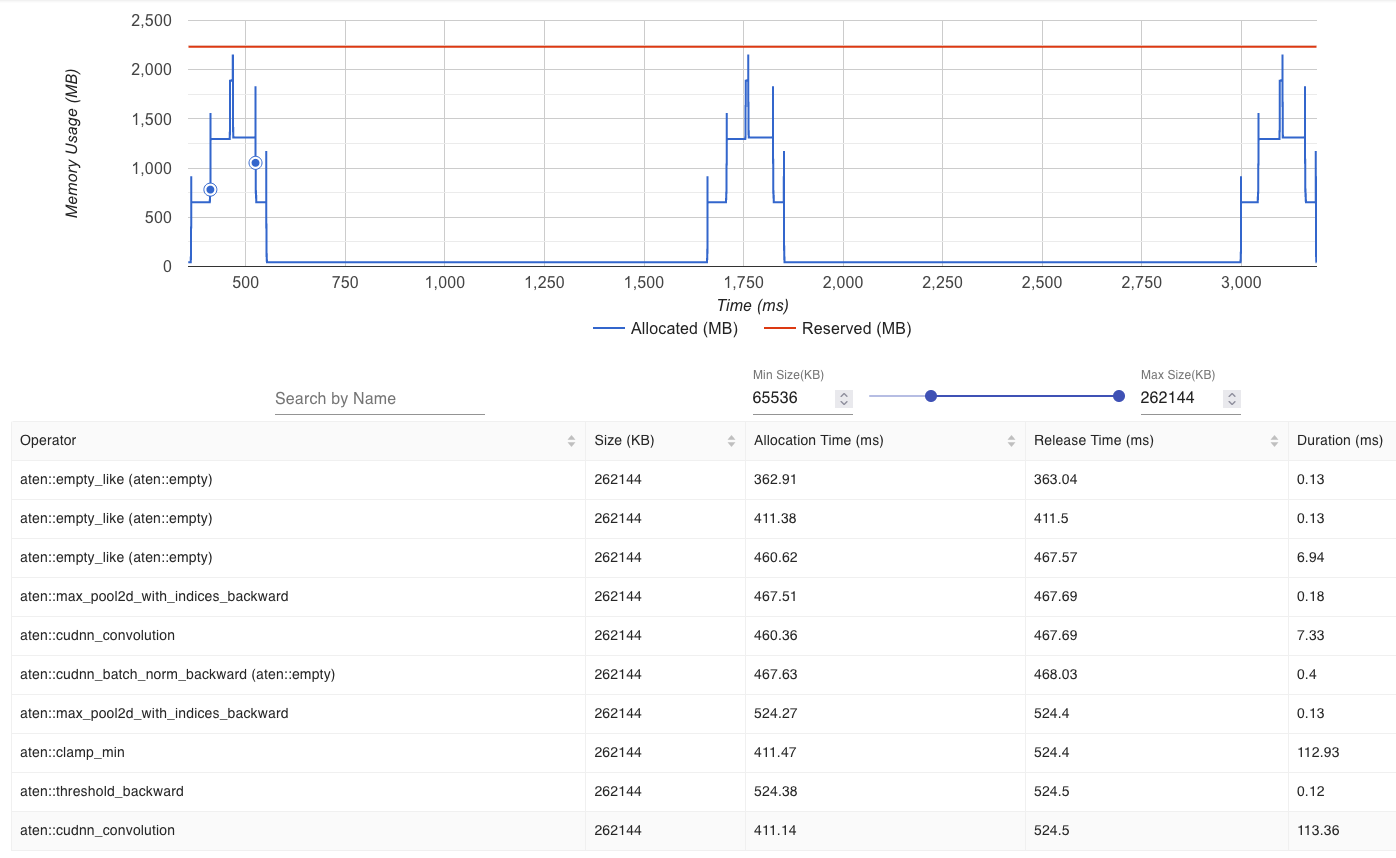
\includegraphics[width=0.85\textwidth]{./assets/scap_gtx1080_profiler-torch_batch-size-64_14650758_memory-view}
\caption[Memory View]{}
\label{fig:scap_gtx1080_profiler-torch_batch-size-64_14650758_memory-view}
\end{figure}

\begin{figure}[H]
\centering
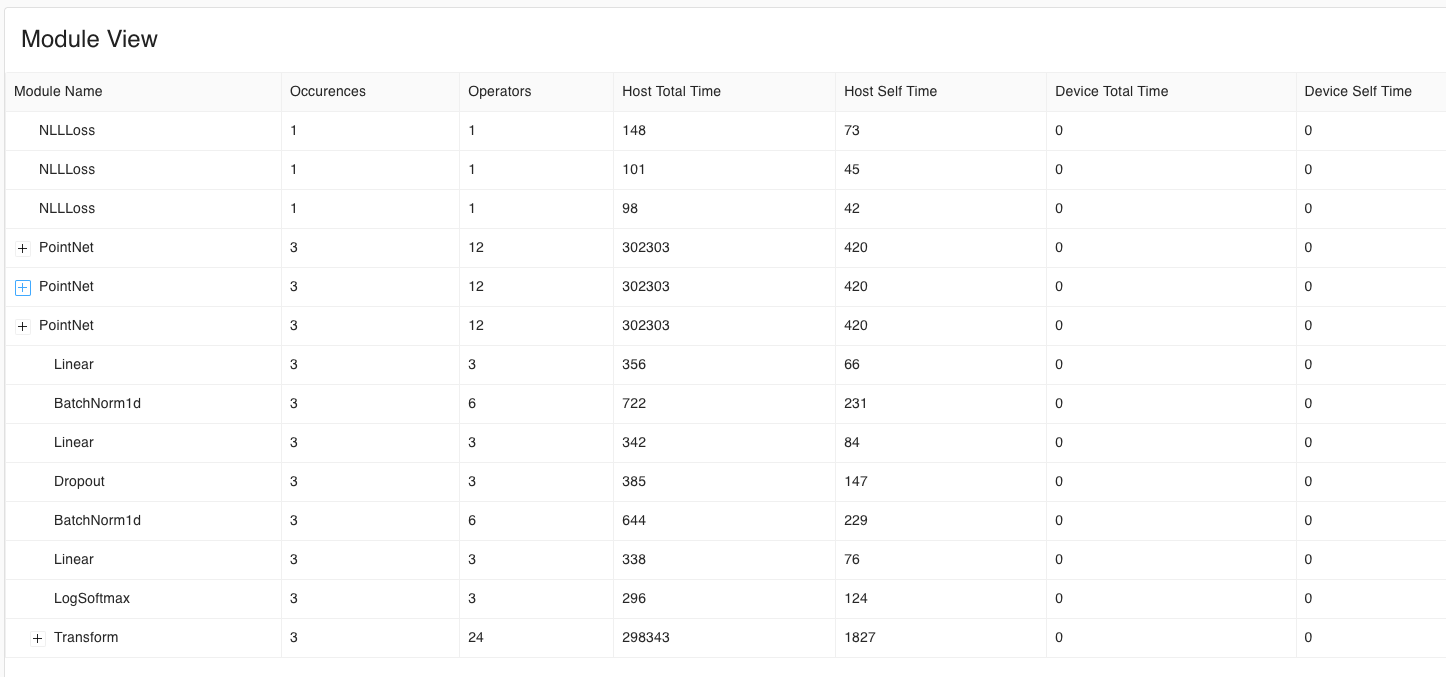
\includegraphics[width=1\textwidth]{./assets/scap_gtx1080_profiler-torch_batch-size-64_14650758_module-view}
\caption[Module View]{}
\label{fig:scap_gtx1080_profiler-torch_batch-size-64_14650758_module-view}
\end{figure}


\section{Code samples}

This is part of the appendix...


\end{document}  
